
\section{Introduction}

% Same as ACRA

%Classification is one of the most widely used instances of supervised  learning, with applications in numerous areas such as spam detection \parencite{spam};  credit scoring, \parencite{scoring}; computer vision \parencite{chen2015handbook}; autonomous driving systems \parencite{gal} and genomics \parencite{genom}, to name but a few. In recent years, the field has experienced an enormous growth becoming a major research area in statistics and machine learning \parencite{efron2016computer}.

Classification is a major research area in machine learning with important applications  in security and cybersecurity, including fraud detection \parencite{bolton2002statistical}: phishing detection \parencite{rakesh}, terrorism \parencite{terror} or cargo screening \parencite{cargo}. An increasing number of processes are being automated through classification algorithms, being essential that these are robust to trust key operations based on their output. State-of-the-art classifiers perform extraordinarily well on standard data, but they have been shown to be vulnerable to adversarial examples, that is, data instances targeted at fooling the underlying algorithms. \textcite{comiter} provides an excellent introduction from a policy perspective, pointing out the potentially enormous security impacts that such attacks may have over systems for filter content, predictive policing or autonomous driving, to name but a few. 

Most research in classification has focused on obtaining more accurate algorithms, largely ignoring the eventual presence of adversaries who actively manipulate data to fool the classifier in pursue of a benefit. Consider 
spam detection: as classification algorithms are incorporated to such task,
spammers learn how to evade them. Thus, rather than sending their spam messages in standard language, they 
 slightly modify spam words (frequent in spam messages but not 
so much in legitimate ones), misspell them or 
change them with synonyms; or they add good words (frequent in legitimate emails but not in spam ones) to fool the detection system. %meaning retained?

Consequently, classification algorithms in critical AI-based systems must be robust against adversarial data manipulations. To this end, they have to take into account possible modifications of input data
due to adversaries.~The subfield of
classification that seeks for algorithms with robust behaviour against adversarial perturbations is known as adversarial classification (AC)
and  was pioneered by \textcite{dalvi2004adversarial}.
%should take into account possible modifications on the behaviour of adversaries so as to be robust against adversarial data manipulations. %
%As a fundamental underlying hypothesis, algorithms rely on the use of independent and identically distributed (iid) data for both the training and test phases. However, security aspects in classification, which form part of the field of adversarial machine learning (AML), questions such iid data hypothesis due to the presence of  adversaries ready to modify the data to obtain a benefit, and, thus, making the training and test distributions differ.
Stemming from their work, the prevailing paradigm 
when modelling the confrontation between classification systems and adversaries has been game theory, see recent reviews by \textcite{BIGGIO2018317} and \textcite{doi:10.1002/widm.1259}. This entails well-known common knowledge hypothesis \parencite{Antos,gameTheoryACriticalIntroduction2004} according to which agents share information about their beliefs and preferences. From a fundamental point of view, this is 
not sustainable in  application areas such as security or cybersecurity,
as participants try to
hide and conceal information.  

After reviewing key developments in game-theoretic approaches to AC in Sections \ref{sec:ac_acr} and \ref{sec:ac_ac}, we cover novel techniques based on adversarial risk analysis (ARA, \textcite{AMLARA}) in Sections  \ref{sec:ac_acra} and \ref{sec:scalable}. Their key advantage is that they do not assume strong common knowledge hypothesis concerning belief and preference sharing, as with standard game theoretic approaches to AML. In this, we unify, expand
and improve upon earlier work in \textcite{naveiro2018adversarial} and
\textcite{gallego2020protecting}.
Our focus is on binary classification
 problems in face only of {\em exploratory attacks}, defined to have influence over operational data but not over training ones. In addition, we restrict our attention to attacks affecting only malicious instances, the so-called \textit{integrity-violation attacks}, the usual context in most security scenarios. We assume that the attacker will, at least, try to modify every malicious instance before the
classifier actually observes it. 
Moreover, attacks will be assumed to be {\em deterministic},
in that we can predict for sure the results of their 
application over a given instance.
\textcite{AdversarialMachineLearning2011} and \textcite{Barreno2006} provide taxonomies of attacks against classifiers. %italics necessary?
%

We first consider approaches in which learning about the adversary is performed in the
operational phase, studying how to robustify generative classifiers against attacks. In certain applications, these  could be very demanding from a computational perspective; for those cases, we present in Section \ref{sec:scalable} an  
approach in which adversarial aspects are incorporated in the training phase.
%to robustify the classifier.
Section \ref{sec:conEx} illustrates the proposed framework
with spam detection and image processing examples.

%%%%%%%%%%%%%%%%%%%%%%%%%%%%%%%%%%
\section{Attacking Classification Algorithms}\label{sec:ac_acr}

%%%%%%%%%%%%%%%%%%%%%%%%%%%%%%%%%%%
\subsection{Binary Classification Algorithms}\label{sec2.1}

In binary classification settings, an agent that we call classifier ($C$, she)
may receive instances belonging to one of two possible  classes denoted, in our context, as malicious ($y=y_1$) or innocent ($y=y_2$).  Instances have  features $x \in \mathbb{R}^d$ whose distribution informs about their class $y$.  Most classification approaches can be typically broken down in two separate stages, the training and operational phases \parencite{bishop2006pattern}.
%
%Features are $d$-dimensional vectors of categorical, ordinal or continuous variables.
%

The first one is used to learn the distribution $p_C(y|x)$, modelling the classifier's beliefs about the  instance class $y$ given its features $x$. 
Frequently, a distinction is introduced 
between {\em generative} and {\em discriminative} models. % \parencite{bishop2006pattern}. 
   In the first case, models $p_C(x|y)$ and $p_C (y)$ are learnt from training data; based on them,
$p_C(y|x)$ is deduced through Bayes formula. Typical examples include 
Naive Bayes \parencite{rish2001empirical} and (conditional) variational autoencoders %\parencite{lopez2017conditional}. %
 \parencite{kingma2014semi}.
%
%uncertainty about the objects' types is modelled through parametric distributions $ p_C(y_i|\beta,x), i=1, 2$. In particular,
In discriminative cases, $p_C(y|x)$ is directly learnt from data.
Within these, an important group of methods uses  
a parameterised function
$f_\beta : \mathbb{R}^d \rightarrow \mathbb{R}^2 $
so that the prediction is given through 
$p_C(y|x,\beta) = \mbox{softmax} (f_\beta (x))[y]$: when $f_\beta (x) = \beta' x$, we recover the logistic regression
model 
\parencite{mccullagh1989generalized}; 
if $f_\beta$ is  a sequence of linear transformations alternating certain nonlinear activation functions,   %, such as Rectified Linear Units (ReLU),
 we obtain a feed-forward neural network \parencite{bishop2006pattern}. 
 Learning depends then on the underlying
methodology adopted.
%
\begin{itemize}
\item In frequentist approaches, training data $\mathcal{D}$ is 
typically used to construct a (possibly regularised) maximum likelihood estimate $\hat{\beta}$, and $p_C(y | \hat{ \beta }, x )$ is employed for classification. Parametric
differentiable models are amenable to training with \emph{stochastic gradient descent}
(SGD) \parencite{bottou2008tradeoffs}  %through parameter updates of the form
%$$
%\beta_{t+1} = \beta_t + \eta \frac{1}{|\mathcal{B}|} \sum_{x \in \mathcal{B}} %\nabla_\beta \log p_C(y|x, \beta_t),
%$$
using a minibatch %$\mathcal{B}$ 
of samples at each iteration. 
This facilitates, e.g.,  training 
deep neural networks with large amounts of
high-dimensional data as 
with images or text data \parencite{10.5555/3086952}.
\item In Bayesian approaches, a prior $p_C (\beta)$ is used to compute the posterior $p_C (\beta | \mathcal{D} )$, given the data $\mathcal{D}$, and the predictive distribution
\begin{equation}\label{MIERDA}
p_C (y | x, \mathcal{D})= \int p_C(y | \beta , x ) p_C (\beta | \mathcal{D} ) d\beta 
\end{equation} 
is used to classify. Given current technology,
in complex environments  
we are sometimes only able to approximate the posterior mode $\hat {\beta}$,
then using $p_C(y | \hat {\beta} , x )$.
\end{itemize}
In any case, and whatever the learning approach adopted, we shall use the notation $p_C (y |x)$. 

The second stage is {\em operational}.
The agent makes class assignment decisions based on $p_C (y |x)$. % $y_C$ perceiving some utility $u_C(y_C,y)$. 
This may be formulated through the influence diagram (ID)
\parencite{evaluatingInfluenceDiagrams1986} in Figure \ref{fig:classification}. {In it, square nodes describe decisions; circle nodes, uncertainties; hexagonal nodes refer to the associated utilities. Arcs pointing to decision nodes are dashed and represent information available when the corresponding decisions are made. Arcs pointing to chance and value nodes suggest conditional dependence.}%Footnote was move here, please check.
%\begin{center}
\begin{figure}[H]
\centering
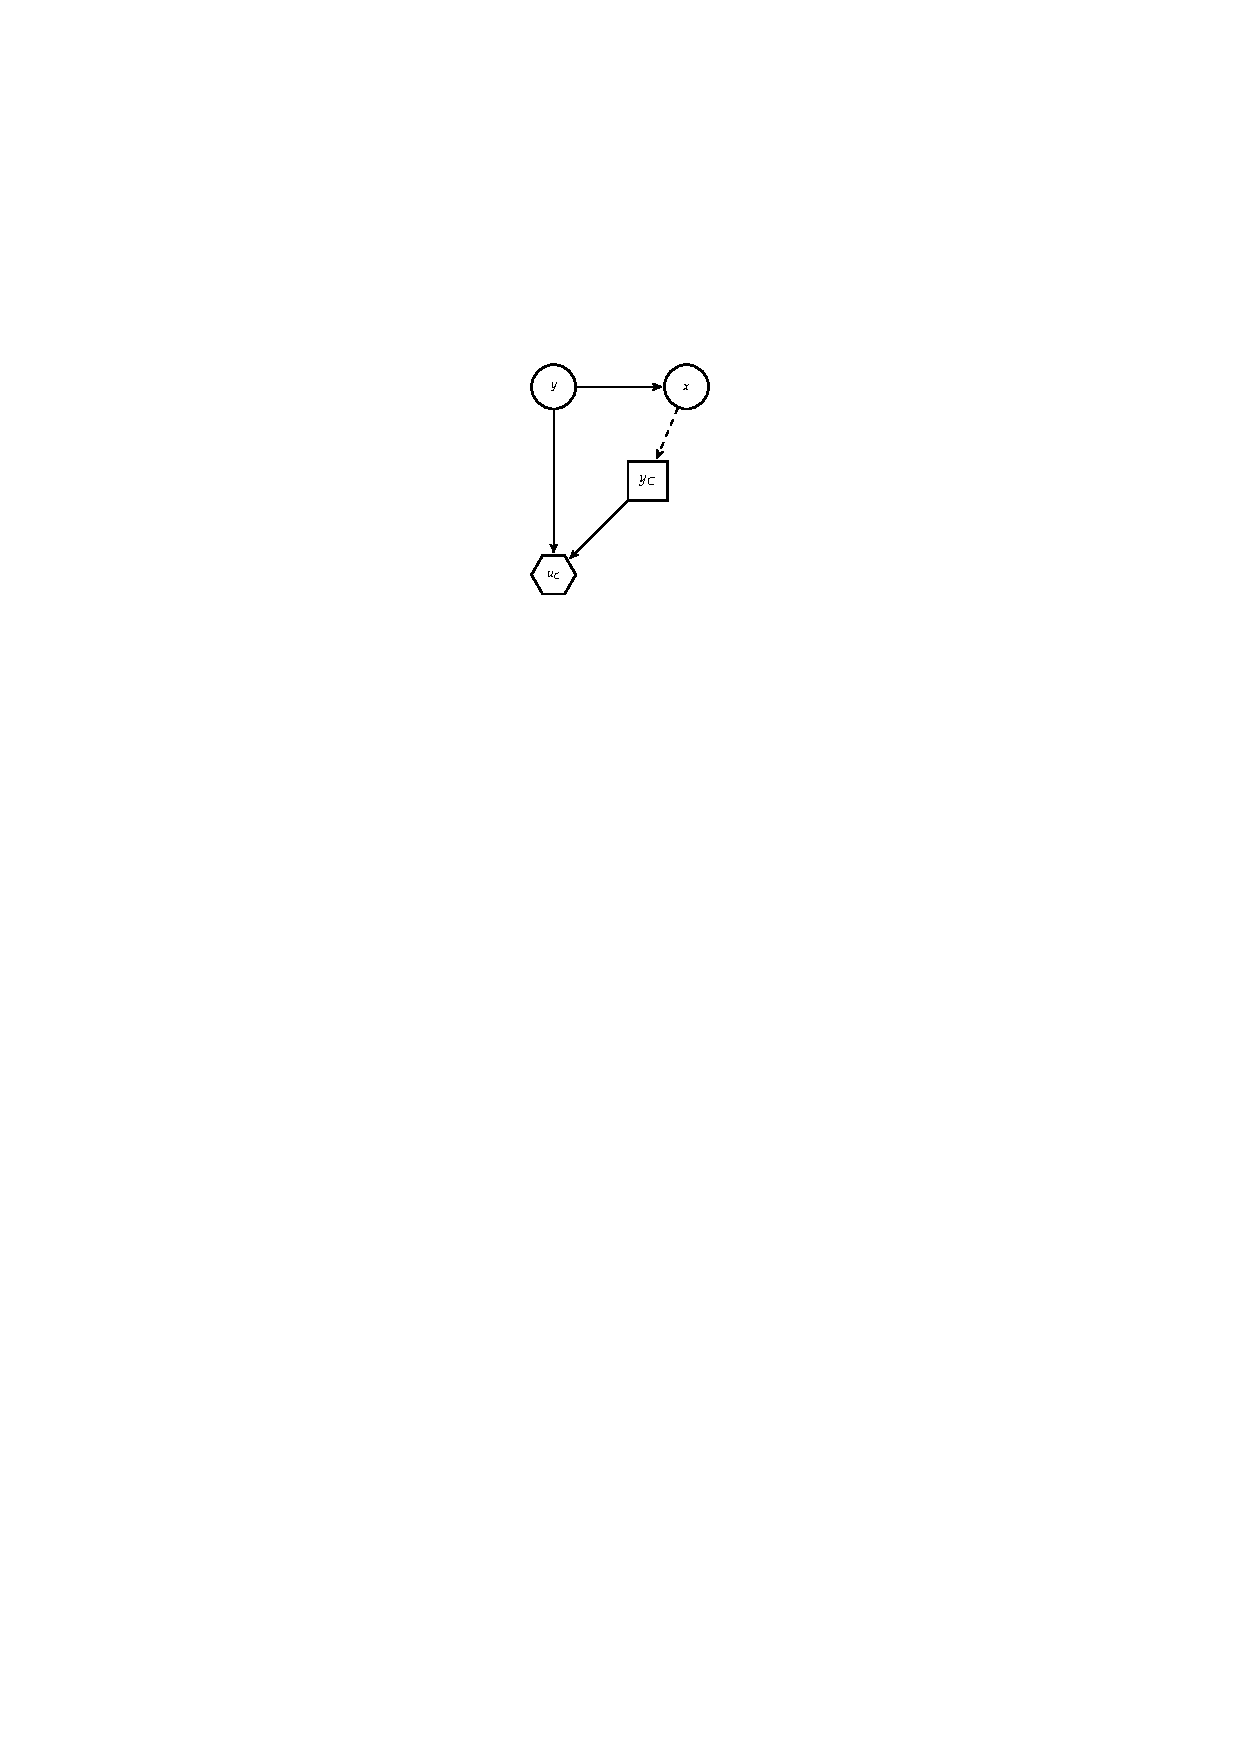
\includegraphics[scale=1]{figures/1.pdf}
\caption{Classification as an influence diagram.} \label{fig:classification}
\end{figure}
%\end{center}
%Consider a classifier $C$ (she) who may receive $k$ types of objects. Their type %is designated with a label $y_i, i=1,...,k$. Objects have features $x$.
 The classifier guess $y_c$ for an observed instance $x$ provides her with a utility $u_C (y_c, y_i)$ when the
 actual class is $y_i$ and she aims at maximising expected utility
 through  
\begin{equation}\label{amarinha}
 \arg\max_{y_c} \sum_{i=1}^2
u_C (y_c , y_i ) p _C (y_i | x ).
\end{equation}
An important example of utility functions is the 0-1 utility: $u_C (y_c, y_i) = \mathbb{I}(y_c = y_i)$, where $\mathbb{I}$ is the indicator function. This leads to deciding based on maximising the
 predictive probability of correct~classification
 %
\begin{equation}\label{seen}
\arg\max_{y_c} \sum_{i=1}^2 \mathbb{I}(y_c = y_i) p_C(y_i|x) = \arg\max_{y_c} p_C(y_c|x).
\end{equation}
%
In general, the 
utility is characterised as
a $2 \times 2$ matrix, whose $ij$-th entry 
represents the utility that the classifier
receives for classifying an instance of true label $j$ as of being of class $i$. This essentially balances the relative importance of false positives and negatives. Consider the case of autonomous driving systems. 
In it, proper classification of identified objects is of
major 
importance. Misclassification errors increase the 
likelihood of incorrect forecasts of an object’s behaviour and an inaccurate assessment of the environment. To minimise the risk of accidents, the system should be very sensitive and react safely when there is uncertainty about the situation. Regrettably, such systems are prone to false-positive emergency identifications that lead to unnecessary reactions. % As an example, 
%attempts to balance the trade-off between system sensitivity and synthetic emergencies were a contributing factor in the 2018 accident wherein an Uber AV killed a pedestrian in Tempe, Arizona. The emergency braking feature of the Volvo XC90 involved was not engaged because of an anti-false-positives policy; instead, the ADS was reliant on the driver to take evasive action who, unfortunately, began braking fractions of a second before impact.


%This is nothing but an affine transformation of the predictive function of the classifier, so this generalization can be straightforwardly adapted in our framework.}

Recall, anyway, that there are classification techniques, such as those based on SVMs, that rather than breaking classification in training and operational stages, directly learn a function that maps features $x$ into labels $y$. Should we like to apply the methodologies described below to this type of classifiers, we would need to produce estimates of $p_C(y|x)$ using their outputs. This can be achieved using calibration techniques such as 
\parencite{platt1999probabilistic} scaling.

 

%%%%%%%%%%%%%%%%%%%%%%%%%%%%%%%%%%%
\subsection{Attacks to Binary Classification Algorithms} \label{sec:att_class}

Consider now another agent called adversary ($A$, he).
He aims at fooling $C$ and make her err in classifying instances to attain some benefit. 
$A$ applies an attack $a$ to the features $x$ leading to $x'=a(x)$, the actual observation received by $C$, which does 
not observe the originating instance $x$.
For notational convenience, we sometimes write $x=a^{-1} (x')$.
%and designate a general transformation from $x$ to $x'$ through $a_{x %\rightarrow x'}$.}
Upon observing $x'$, $C$ needs to determine the instance  class. 
%In adversarial settings, another agent, called adversary ($A$, he), chooses an
%attack $a$ which, applied to the features $x$, leads to the perturbed data $x'=a(x)$ that are actually observed by $C$. 
%When $y=-$, $x' = x$ and the 
%classifier makes no mistakes in her classification. However, when $y=+$, $x' = %a(x)$ an adversary
As we next illustrate, an adversary unaware classifier
may incur in gross mistakes if she classifies based on features $x'$, instead of the original ones.
%, implicitly assuming that the observed instance is the same as %the originating one.
%%%%%%%%%%%%%%%%%%%%%%%%%

%%%%%%%%%%%%%%%%%%%%%%%%%%%%%%%%%%%%%
\paragraph{Example.} Attacks to spam detection systems will be illustrated with experiments carried out with the UCI Spam Data Set \parencite{spambase1999}.
This set contains data from 4601 emails, out of which $39.4 \%$ are spam. For classification purposes, we represent each email through 54 binary variables indicating the presence (1) or absence (0) of 54 designated words in a dictionary.

Table \ref{tab:cleanVSattack} presents the performance
of four standard classifiers ({\em  Naive Bayes, logistic regression, neural net} and {\em  random forest}) based on a 0--1 utility function, against tainted and untainted data. The neural network model is a two layer one. The logistic regression is applied with L1 regularisation; {this  is equivalent to performing maximum a posteriori estimation in a logistic regression model with a Laplace prior \parencite{park2008bayesian}}. % Footnote was move here, please check.
Means and standard deviations of accuracies are estimated via repeated hold-out validation over ten repetitions~\parencite{kim2009estimating}.
%Note that SVMs do not produce estimates of $p_C(y_c|x)$ directly. To generate such probabilistic outputs we use Platt scaling \parencite{platt1999probabilistic}. 
%
%Consider classification with Support Vector Machines (SVM) \parencite{moguerza}, based %on the $\ell_1$ and $\ell_2$ norms.  A 5-fold cross validation was undertaken to %choose the best value for the SVM parameter $C \in \{2^{-12}, 2^{-11}, \dots, %2^{11}, 2^{12}\}$ with a clean dataset. Results are reported in Table %\ref{tab:SVMcleanVSattack}. The accuracy (ACC) and the area under the curve (AUC) %are means over the five iterations; $C^*$ reports the smallest value $C$ for which %ACC and AUC coincid.
% \pagebreak 
% \begin{table}[htbp]
% 	\centering
% 	\begin{tabular}{ccccc}
% 		\toprule
% 		Classifier & Acc. Unt. & Acc. Taint. \\
% 		\hline
% 		Naive Bayes   & $0.888 \pm 0.004$ & $0.680 \pm 0.030$         \\
% 		Log Reg Clas  & $0.930 \pm 0.005$    & $0.662 \pm 0.005$      \\  
% 		Log Reg Bay  &   $0.930 \pm 0.002$    & $0.615 \pm 0.004$            \\
% 		Neural Net  &      $0.931 \pm 0.001$     &     $0.594 \pm 0.009$          \\
% 		Random Forest   &    $0.944 \pm 0.002$  &    $0.693 \pm 0.005$           \\
% 		\bottomrule
% 	\end{tabular}%
% 	\caption{Accuracy comparison (with precision) 
% 	of five classifiers on clean
% 	(untainted) and attacked (tainted) data.}
% 	\label{tab:cleanVSattack}%
% \end{table}%


\begin{table}[H]
\caption{Accuracy comparison (with precision) 
 	of four classifiers on clean
 	(untainted) and attacked (tainted) data.}
	\centering
	\begin{tabular}{ccccc}
		\toprule
		\textbf{Classifier} & \textbf{ Acc. Unt.} & \textbf{Acc. Taint.}  \\
		\midrule
		Naive Bayes   & $0.891 \pm 0.003$ & $0.774\pm 0.026$  \\
		Logistic Reg.  & $0.928 \pm 0.004$ & $0.681 \pm 0.009$    \\  
		%SVM  & $0.942 \pm 0.003$  &   $0.694 \pm 0.007$           \\
		Neural Net & $0.905 \pm 0.003$ &      $0.764 \pm 0.007$       \\
		Random Forest  & $0.946 \pm 0.002$  &    $0.663 \pm 0.006$       \\
		\bottomrule
	\end{tabular}%
	
	\begin{tabular}{@{}c@{}} 
\multicolumn{1}{p{\textwidth -.88in}}{\footnotesize Observe the important loss in accuracy of the four classifiers, showcasing a major degradation in performance of adversary unaware classifiers when facing attacks.}
\end{tabular}
	\label{tab:cleanVSattack}%
\end{table}

%\noindent The first column provides the norm used; the second one, the data set %used; the third, the value of $C^*$; the fourth, the ACC; finally, the fifth one, %the AUC. For attacked data, the ACC and AUC are reported using $C^*$ for clean %data, as we assume that the classifier is attacker unaware. As we can appreciate, %the 
%loss in performance is greater than $10\%$ in both cases. 


%%%%%%%%%%%%%%%%%%%%%%%%%%%%%%%%%%%%%%%%%%%%%%%%%%
\section{Adversarial Classification: Game-Theoretic Approaches}\label{sec:ac_ac}

As exemplified, an adversary unaware classifier may be fooled into issuing wrong classifications leading to severe performance deterioration. Strategies to mitigate this problem are thus needed. These may be based on 
building models of the attacks likely to be undertaken by the adversaries and enhancing classification algorithms to be robust against such attacks.% We focus on Bayesian classification approaches but the ideas extend to classical ones.

For this, the ID describing the classification problem (Figure \ref{fig:classification}) is augmented to incorporate adversarial decisions, leading to a biagent influence diagram (BAID) \parencite{Banks},
 Figure \ref{fig:jointProblem}. { In it, grey nodes refer to elements solely affecting $A$'s decision; white nodes to issues solely pertaining to $C$'s decision; striped nodes affect both agents' 
decisions}. %Footnote was move here, please check.
We only describe the new elements. 
First, the adversary decision is represented through node $a$ (the chosen attack). The impact of the data transformation over $x$ implemented by $A$ is described through node $x'$, the data actually observed by the classifier; the 
corresponding node is deterministic 
(double circle) as we assume deterministic attacks.
Finally, the utility of $A$ is represented with node $u_A$,
with form  $u_A(y_c, y)$, when $C$ says $y_c$ and the actual label is $y$.
% and the attack is $a$, which has an implementation cost. 
%Thus, 
 We assume that attack implementation has negligible
costs.
As before, $C$ aims at maximising her 
expected utility; $A$ also aims at maximising his expected utility 
trying to confuse the classifier (and, consequently, reducing her 
expected utility). % Footnote was move here, please check.
%\begin{center}
\begin{figure}[H]
\centering
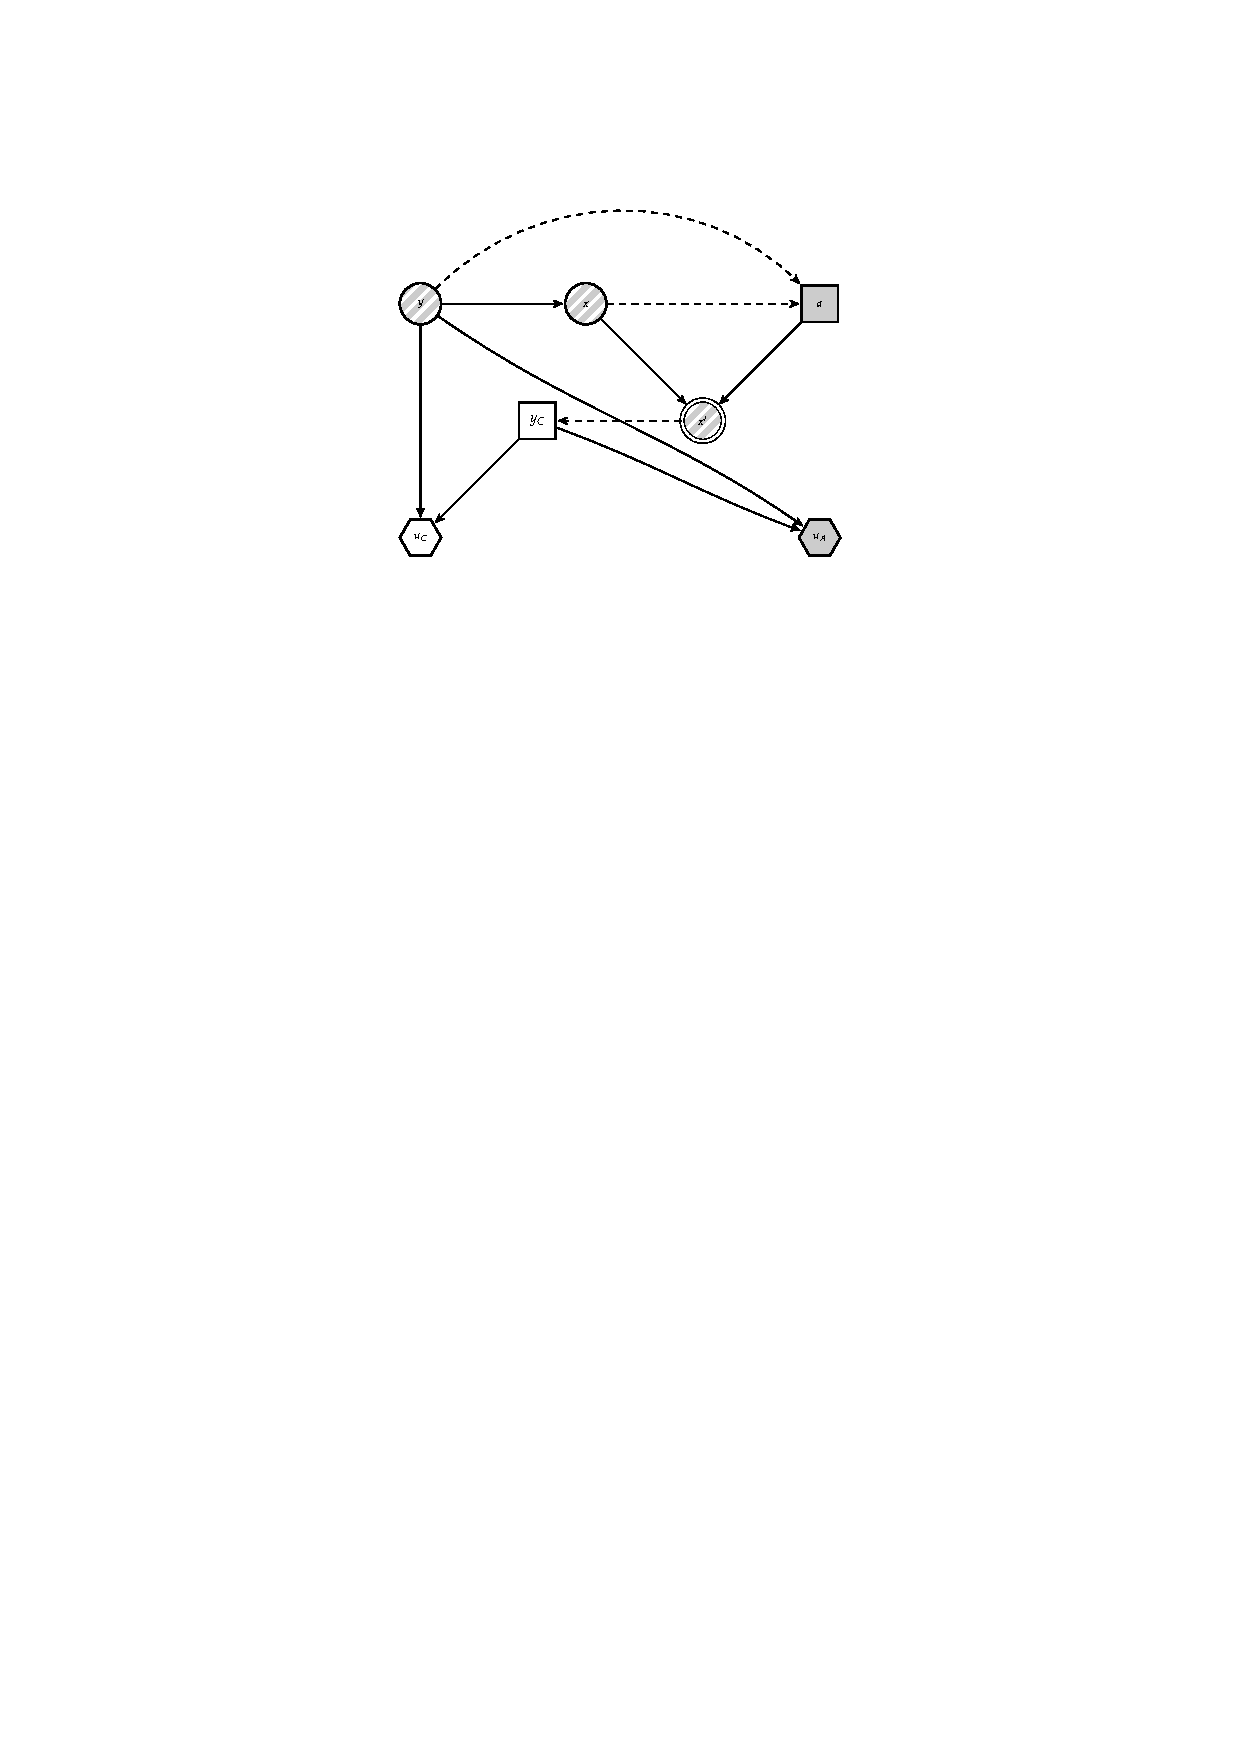
\includegraphics[scale=1]{figures/2.pdf}
\caption{Adversarial classification as a biagent influence diagram.}\label{fig:jointProblem}
\end{figure}
%\end{center}

%%%%%%%%%%%%%%%%%%%%%%%%%%%%%%%%%%%%%%
\subsection{Adversarial Classification. The Pioneering Model.%Reference citations are not allowed in the title. Please move it the main text.
}
\textcite{dalvi2004adversarial} provided a pioneering approach to enhance classification algorithms when an adversary is present, calling it adversarial classification (AC).
 Because of its importance,
we briefly review it, using our notation. 
The authors view the problem as a game between a classifier $C$ and an adversary $A$,
%. The classifier aims at finding an optimal classification strategy against $A$'s optimal attacking strategy. However, computing Nash equilibria \parencite{ozdaglar2011network} in such general games becomes overly complex. Therefore, they propose 
using the following forward myopic proposal.


\begin{enumerate}
\item \textit{C} first assumes that data is untainted and computes her optimal classifier through (\ref{amarinha}).
%\begin{equation} \label{dalviC}
%    \argmax_{y_c} \sum_{i=1}^2 u(y_c, y_i) p_C(y_i |x)
%\end{equation}
\textcite{dalvi2004adversarial} focuses on  a utility sensitive Naive Bayes algorithm \parencite{elkan2001foundations}.
\item Then, assuming that \textit{A} has complete information about the classifier's elements (a common knowledge
assumption)
and that $C$ is not aware of his presence, the authors 
compute $A$'s optimal attack. 
To that end, they propose solving the integer programming  problem
\begin{align} \label{dalviA}
    \begin{split}
        \min & \left \lbrace \sum_{X_i \in \mathcal{X}_C} \sum_{x'_i \in \mathcal{X}_i} \mathcal{C}(x_i, x'_i) \delta _{i, x'_i} \right \rbrace\qquad {\rm s.t.} \\
        & \sum_{X_i \in \mathcal{X}_C} \sum_{x'_i \in \mathcal{X}_i} \left ( \log \frac{p_C(x_i|y_1)}{p_C(x_i|y_2)} - \log \frac{p_C(x'_i|y_1)}{p_C(x'_i|y_2)} \right ) \delta _{i, x'_i} \geq gap(x) .
    \end{split}
\end{align}
where $\mathcal{X}_C$ is the set of features the classifier uses for making her decision and $X_i$, the $i$-th feature, with original value $x_i \in \mathcal{X}_i$, assumed to be discrete. %, providing the least cost feature 
%transformation leading to a change in the classification.
 $\delta_{i, x'_i}$ is a binary variable adopting value 1 when feature $X_i$ is changed from $x_i$ to $x'_i$, being $\mathcal{C}(x_i, x'_i)$ the cost of such change. 
 %; and 0, otherwise. 
It is easy to see that problem \eqref{dalviA} reflects the fact that the adversary tries to minimise the cost of modifying an instance, provided that such modification induces a change in the classification decision.

%Thus, the
%objective function in \eqref{dalviA}, expresses that the adversary tries to change features minimizing his total cost. 
%In turn, the constraint ensures that feature modification will induce a change in the classification decision. It is easy to see that the classifier will declare an instance as malicious if
%
%\begin{equation*}
%    gap(x)= \log \frac{p_C(x|y_1)}{p_C(x|y_2)} -  \log \frac{u_C(y_2, y_2) - u_C(y_1, y_2)}{u_C(y_1, y_1) - u_C(y_2, y_1)} > 0.
%\end{equation*}
%
%We call the left term of this expression $gap(x)$.
%The adversary is thus interested in modifying the features of malicious instances from $x$ to $x'$, such that they are classified as legitimate, that is $gap(x') < 0$. A feature modification induces a change on the log odds, from $\log \frac{p_C(x|y_1)}{p_C(x|y_2)}$ to $\log \frac{p_C(x'|y_1)}{p_C(x'|y_2)}$. It is straightforward to see that, in order for the new instance to have $gap(x') < 0$, old 
%minus new odds must surpass $gap(x)$, as reflected by the constraint in  \eqref{dalviA}.


\item Subsequently, the classifier, assuming that $A$ implements the previous attack (again a common knowledge assumption) and that the training data is untainted, deploys her optimal classifier against it:
she chooses $y_c$ maximising $\sum_{i=1}^2 u_C(y_c, y_i) p_C(y_i |x')$, her posterior expected utility given that she observes the possibly modified instance $x'$. This is equivalent to optimising 
%
\begin{eqnarray}\label{dalviCK}
u_C (y_c, y_1) p_C(x' |y_1) p_C(y_1) + u_C (y_c, y_2) p_C(x' |y_2) p_C(y_2).
\end{eqnarray}
%
Estimating all these elements is straightforward, except for $p_C(x' \vert y_1)$. Again, appealing to a common knowledge assumption, the authors assume that the classifier, who knows all the adversary's elements, can solve 
\eqref{dalviA} and compute $x' = a(x)$, for each $x$ the adversary may receive.~Thus
%
\begin{eqnarray*} 
p_C(x' |y_1) = \sum_{x \in \mathcal{X}'} p_C (x \vert y_1) p_C (x' \vert x, y_1)
\end{eqnarray*}
where $\mathcal{X}'$ is the set of possible instances leading to the observed one and $p_C(x' \vert x, y_1) = 1$ if $a(x) = x'$ and 0 otherwise.
%Estimating $p(y_1)$ (and $p(y_2)$) is simple,
%based on training data, clean by assumption. In addition, as the authors assume that legitimate instances are not modified, $p_C(x' |y_2) = p_C(x |y_2)$ which can be estimated as well from training data. To estimate $p_C(x' \vert y_1)$, the authors appeal yet again to a common knowledge assumption: if the adversary receives instance $x$, then the classifier, who knows all its involved elements, can solve problem \eqref{dalviA} and compute $x' = a(x)$. Thus
%
%\begin{eqnarray*} 
%p_C(x' |y_1) = \sum_{x \in \mathcal{X}'} p_C (x \vert y_1) p_C (x' \vert x, y_1)
%\end{eqnarray*}
%where $\mathcal{X}'$ is the set of possible instances leading to the observed one and $p_C(x' \vert x, y_1) = 1$ if $a(x) = x'$ and 0 otherwise.
%
\end{enumerate}
%
The procedure could continue for more stages.
However, \textcite{dalvi2004adversarial} considers sufficient to use these three.


As presented (and the authors actually stress this
in their paper), very strong common knowledge assumptions are made: all parameters of both players are known to each other. Although standard in game theory, such  assumption is unrealistic in the security scenarios  
typical of AC.



%{\bf Note that if the above mentioned game-theoretic common knowledge assumptions held, $C$ would be able to compute the set of instances that, with probability 1, $A$ would change to $x'$: we would know $A$'s beliefs and preferences and, therefore, would be able to compute the attacks he is actually implementing. Thus, we find out that for those potential attacks, $p_C(a_{x \rightarrow x'} |x,+)$ would be 1, and 0 for every other. Then, the model would just take into account instances with probability 1, ignoring the others.}

%%%%%%%%%%%%%%%%%%%%%%%%%%%%%%%%%%%%%%%
\subsection{Other Adversarial Classification Game-Theoretic Developments}\label{sec:other_AC}

In spite of this, stemming from 
\textcite{dalvi2004adversarial}, AC has been predated by game-theoretic approaches, as reviewed in \textcite{biggio2014security} or \textcite{li2014feature}.
Subsequent attempts have focused on analysing attacks over classification algorithms and assessing their robustness against them, %, e.g.\ \parencite{adversarialLearning2005}, \parencite{Barreno2006} or \parencite{zhou2012adversarial}.
under various assumptions about the adversary. Regarding attacks, these have been classified as {\em white box}, when
the adversary knows every aspect of the defender's system
like the data used, the algorithms and the entire feature space; 
{\em black box}, that assume limited capabilities for the adversary, e.g., he is able to send membership queries to the classification system as in
\textcite{adversarialLearning2005}; and, finally,
{\em gray box}, which are in between the previous ones, as in \textcite{zhou2012adversarial}
where the adversary, who has no knowledge about the data and the algorithm used
seeks to push his malicious instances
as innocent 
ones, thus assuming that he is able to estimate such instances and has knowledge about the feature space. 

Of special importance in the AC field, mainly 
within the deep learning community, are the so called {\em adversarial 
examples} \textcite{goodfellow2014explaining} which may be formulated in game-theoretic terms as 
optimal attacks to a deployed classifier, requiring, in principle,
precise knowledge about the model used by the classifier.
To create such examples, $A$ finds the best attack which 
leads to perturbed data instances obtained from solving
problem   
$
\min_{\| \delta \| \leq \epsilon} \widehat{c}_A(h_{\theta} (a(x)), y),
$
 with $a(x) = x + \delta$, a  perturbation of the original data instance $x$; 
$h_{\theta} (x)$, the output of a predictive model with parameters $\theta$;
and
$\widehat{c}_A(h_{\theta} (x), y)$ the adversary's cost when instance $x$ of class $y$ is classified as of being of  class $h_\theta (x)$. This cost is usually taken to be $-\widehat{c}_D(h_{\theta} (x), y)$, where $c_D$ is the defender's cost.
The Fast Gradient Signed Method  (FGSM, \textcite{goodfellow2014explaining}) and related attacks in the literature \parencite{vorobeichikantar} assume that the attacker
has precise knowledge of the underlying model and parameters of the involved classifier, 
  debatable in most security settings.

A few methods have been proposed to robustify classification algorithms in adversarial settings. Most of them have focused on application-specific domains, as \textcite{Kocz2009FeatureWF} on spam detection. \textcite{Vorobeychik:2014:ORC:2615731.2615811} study the impact of randomisation schemes over classifiers against adversarial attacks proposing an optimal randomisation scheme as best defence.
 To date, 
\emph{adversarial training} (AT) \parencite{madry2018towards}
is one of the most promising defence techniques:
 it trains the defender model using attacked samples,
solving the~problem
%
\begin{equation*}
    \min_{\theta} \mathbb{E}_{(x,y) \sim \mathcal{D}} \left[ \max_{\| \delta_x \| \leq \epsilon} \widehat{c}_D(h_{\theta} (a(x)), y) \right],
\end{equation*}
%
thus minimising the empirical risk of the model under worst case perturbations of the data $\mathcal{D}$.
AT can be formulated as a zero-sum game. The inner maximisation problem is solved through project gradient descent (PGD) with iterations 
$
x_{t+1} = \Pi_{B(x)} (x_t - \alpha \nabla_x  \widehat{c}_A(h_{\theta} (x_t), y)),
$
where $\Pi$ is a projection operator ensuring that the perturbed input falls within an acceptable boundary $B(x)$,  and $\alpha$ is an intensity hyperparameter referring to the attack strength. After $T$ PGD iterations, set $a(x) = x_T$ and optimise with respect to $\theta$.   Other attacks that use gradient information are deepfool \textcite{moosavi2016deepfool}, yet \textcite{madry2018towards} argue that the PGD attack is the strongest one based only on gradient information from the target model. However, there is evidence that it is not sufficient for full defence in neural models since it is possible to perform attacks using global optimisation routines, such as the \emph{one pixel attack} from \textcite{su2019one} or \textcite{gowal2018ibp}.% The complexity of the attack depends on the chosen norm.

%for instance, if we resort to small perturbations under $\ell_\infty$  norm, the update simplifies to
%$
%x := x - \epsilon\,\mbox{sign} \nabla_x  \widehat{c}_A(h_{\theta} (x), y),
%$
%making it attractive because of its low computational burden. The $\ell_2$ norm can also be considered, leading to updates
%$
%x := x - \epsilon\,\frac{ \nabla_x  \widehat{C}_A(h_{\theta} (x), y)}{\| \nabla_x  \widehat{C}_A(h_{\theta} (x), y) \|_2}.
%$
%Second, \emph{adversarial logit pairing} (ALP), \parencite{kannan2018adversarial}, another defence strategy that encourages the logits of the model to be the same for both natural and adversarial inputs.


Other approaches have focused on improving the game theoretic model in \textcite{dalvi2004adversarial}. However, to our knowledge, none has been able to overcome the above mentioned unrealistic common knowledge assumptions, as may be seen in recent reviews by \textcite{BIGGIO2018317} and \textcite{doi:10.1002/widm.1259}, who point out the importance of this issue. As an example, \textcite{kantarciouglu2011classifier} use a Stackelberg game in which both players know each other's payoff functions. Only \textcite{grosshans2013bayesian} have attempted to relax common knowledge assumptions in adversarial regression settings, reformulating the corresponding problem as a Bayesian game. 


%%%%%%%%%%%%%%%%%%%%%%%%%%%%%%%%%%%%%%%%%%%%%%%%%%%%%%
%%%%%%%%%%%%%%%%%%%%%%%%%%%%%%%%%%%%%%%%%%%%%%%%%%%%
\section{Adversarial Classification: Adversarial Risk Analysis Approaches}\label{sec:ac_acra}

Given the above mentioned issue, we provide ARA solutions to AC.
We focus first on modelling the adversary's problem in
the operation phase. We present the classification problem faced by $C$ as a Bayesian decision analysis problem in Figure \ref{fig:classifierProblem}, derived from Figure \ref{fig:jointProblem}. In it, $A$'s decision appears as random to the classifier, since she does not know how the adversary will attack
the data. {For notational convenience, when necessary we distinguish between random variables and realisations using upper and lower case letters, respectively; in particular, we denote by $X$ the random variable referring to the original instance (before the attack) and $X'$ that referring to the possibly attacked instance. 
$\hat{z}$ will indicate an estimate of $z$.}%Footnote was move here, please check.
%\begin{center}
\begin{figure}[H]
\centering
%\subfloat[Classifier problem \label{fig:classifierProblem}]
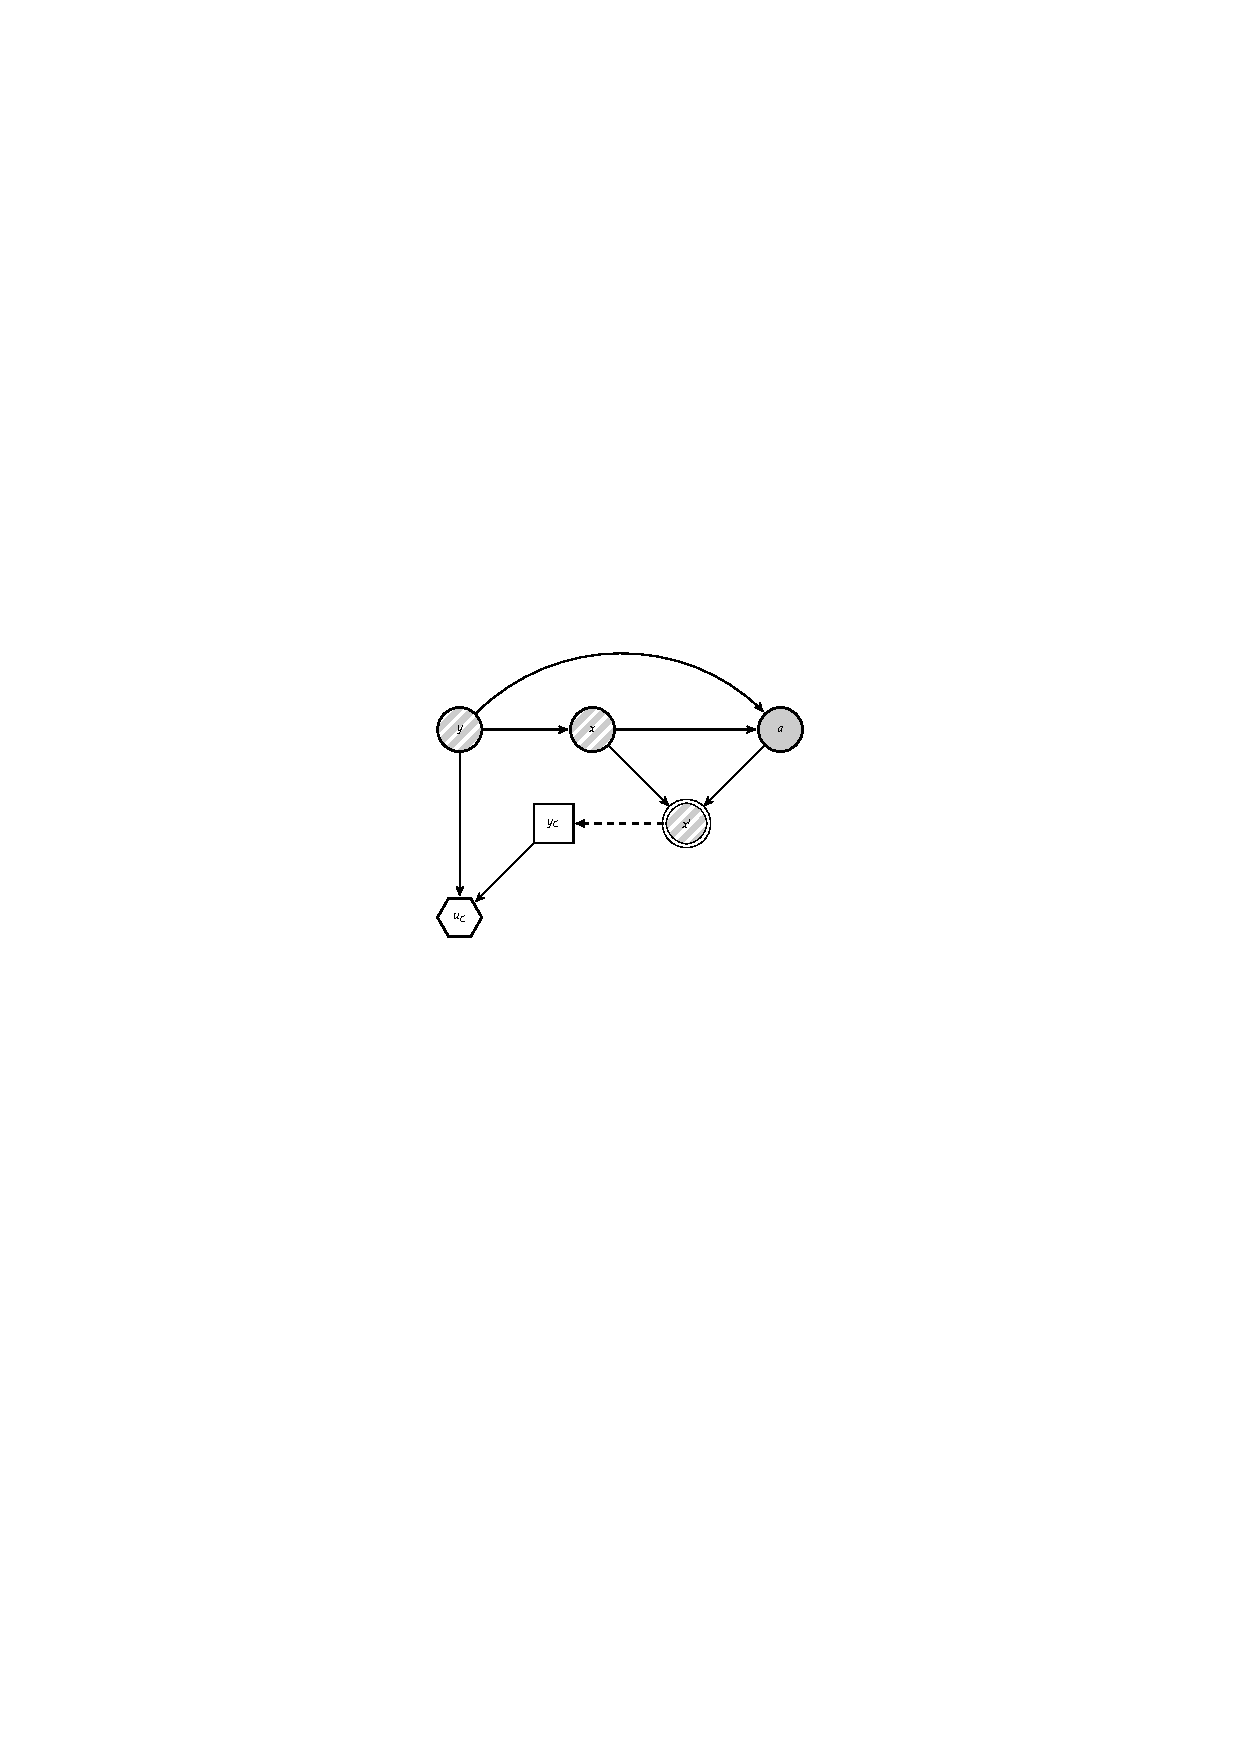
\includegraphics[scale=1]{figures/3.pdf}
\caption{Classifier problem.}
\label{fig:classifierProblem}
\end{figure}
%\end{center}

An adversary unaware classifier would classify the observed instance $x'$ based on
\begin{equation}\label{valdokk}
\arg\max_{y_c} \sum_{i=1}^2  u_C (y_c , y_i ) p_C (y_i | X = x ').
\end{equation}
This leads to performance degradation as reflected in Section \ref{sec:att_class}.
In contrast, an adversary aware classifier would use
\begin{equation}\label{valdosurf}
\arg\max_{y_c} \sum_{i=1}^2  u_C (y_c , y_i ) p_C (y_i | X' = x ').
\end{equation}
In the adversary unaware case, $p_C (y_i | X = x ')$ is easily estimated using the training data. However, estimating 
the probabilities    $p_C (y_i | X' = x ')$ is harder, as it entails modelling how the adversary will modify the original instance $x$, which is unobserved. Moreover,  recall that common knowledge is not available, so we actually lack $A$'s beliefs and preferences. ARA helps us in modelling our uncertainty about them. In doing so, 
 robustness is typically enhanced.
We discuss two strategies depending on whether we use generative or discriminative classifiers as base models. 

%to compute $p (y_i | X' = x ')$
%However, we do not know the attack $a$ (or, more generally, the originating $x$).

%But common knowledge is not available, so we actually lack $A$'s beliefs and preferences. ARA models our uncertainty around them. As we shall see, in doing so we enhance model robustness. 

%%%%%%%%%%%%%%%%
\subsection{The Case of Generative Classifiers}

Suppose first that a generative classifier is required. As training data is clean by assumption, we can estimate $p_C (y)$ (modelling the classifier's beliefs about the {class} distribution) and $p_C (X=x|y)$ (modelling her beliefs about the feature distribution given the {class} when $A$ is not present). In addition, assume that when $C$ observes $X' = x'$, she can estimate the set $\mathcal{X}'$ of original instances $x$ potentially leading to the observed $x'$.  As
later discussed,
in most applications this will typically be a very large set.
When the feature space is endowed with a metric $d$,
an approach to approximate ${\cal X}'$ would be to consider
$%\label{valdo}
{\cal X}'= \{ x : d(x,x')<\rho \}
$ 
 for a certain threshold $\rho$. We will now survey the approach presented in \textcite{naveiro2018adversarial}.

%Moreover, as we only consider deterministic integrity violation transformations, we have that $p_C(a|x, -)$ $= I(a = \textit{id})$, where \textit{id} stands for the identity attack leaving $x$ unchanged and $I$ is the indicator function.

%Suppose for the moment that we are able to assess $p_C(a|x, y)$, portraying $C$'s beliefs about $A$'s action, given $x$ and $y$. We assume also that $C$ is able to approximate the set $\mathcal{A}(x)$ of possible attacks over a given instance $x$.

Given the above, when observing $x'$ the classifier should choose the class with maximum posterior expected utility (\ref{valdosurf}).
%
%\begin{equation}\label{hastael26}
%%    c(x') = \argmax_{y_c} \sum_{i=1}^2 u(y_c, y_i) p(y_i|X'=x'). 
%\end{equation}
%
Applying Bayes formula, and ignoring the denominator, 
which is irrelevant for optimisation purposes, %allows us to use the basic generative ingredients. Consequently, 
she must find the class %$y^*_c(x')$ solving
%
\begin{eqnarray}\label{fene}
   y^*_c(x') &=& \argmax_{y_c} \sum_{i=1}^2 u_C(y_c, y) p_C (y_i) p_C (X'=x'|y_i) \nonumber \\
    &=& \argmax_{y_c} \sum_{i=1}^2  u_C(y_c, y_i) p_C (y_i) 
    \left[ \sum_{x \in \mathcal{X}'} p_C (X' = x'\vert X=x, y_i) p_C (X=x \vert y_i)\right] .   
\end{eqnarray}
%
In such a way, $A$'s modifications are taken into account through the probabilities $p_C(X' = x'\vert X=x, y)$.  
At this point, recall that the focus is restricted to integrity violation attacks.
% Without loss of generality, we denote as $y_1$ the malicous class and $y_2$ the innocent one. Obviously
Then, $p_C(X' = x'\vert X=x, y_2) = \delta(x'-x)$ and problem
 (\ref{fene}) becomes 
%
\begin{eqnarray} \label{pis}
   &\argmax_{y_c} \bigg[ u_C(y_c, y_1) p_C(y_1)  \sum_{x \in \mathcal{X}'} p_C(X' = x'\vert X=x, y_1) p_C(X=x \vert y_1) \nonumber \\
   & + u_C(y_c, y_2) p_C(y_2) p_C(X=x' \vert y_2)\bigg].
\end{eqnarray} % \label{naron}
%
% Finally, as we just deal with deterministic attacks,
% it becomes  
% %
% \begin{eqnarray}
%   &\argmax_{y_c} \bigg[ u_C(y_c, y_1) p_C(y_1)  \sum_{x \in \mathcal{X}'} p_C(a_{x \rightarrow x'} |x,y_1) p_C(x \vert y_1) \nonumber \\
%   & + u_C(y_c, y_2) p_C(y_2) p_C(x \vert y_2)\bigg], \label{pis}
% \end{eqnarray}
%
%where $p_C(a_{x \rightarrow x'} |x,y_1)$ designates the probability that the attacker executes attack $a_{x \rightarrow x'}$, when he receives $(x,y_1)$. 
%Note that dealing with random attacks would require summing over all possible attacks connecting $x$ and $x'$.

Note that should we assume full common knowledge, we would know $A$'s beliefs and preferences and, therefore, we would be able to 
solve his problem exactly: when $A$ receives an instance $x$ from class $y_1$, we could compute the transformed instance. In this case, $p_C(X'|X=x,y_1)$ would be 1 just for the $x$ whose transformed instance coincides with
that observed by the classifier and 0, otherwise. Inserting this 
 in \eqref{pis}, we would recover Dalvi's formulation \eqref{dalviCK}.
However, common knowledge about beliefs and preferences does not hold. 
Thus, when solving $A$'s problem we have to take into account our uncertainty about his elements and, given that he receives an instance $x$ with label $y_1$, we will not be certain about the attacked output $x'$.
This will be reflected in our estimate $p_C(x' |x,y_1)$ which will not be 0 or 1 as in Dalvi's approach (stage 3). With this estimate, we would solve problem \eqref{pis}, summing $p_C(x|y_1)$ over all possible originating instances, with each element weighted by $p_C(x' |x,y_1)$.

To estimate these last distributions, we resort to $A$'s problem, assuming that this agent aims at modifying $x$ to maximise his expected utility by making $C$ classify malicious instances as innocent. The decision problem faced by $A$ is presented in Figure \ref{fig:adversaryProblem}, derived from Figure \ref{fig:jointProblem}. In it, $C$'s decision appears as an uncertainty to $A$. 
%$p_C(a_{x \rightarrow x'} |x,y_1)$ will not be 0 or 1, as we will model our uncertainty about the attacker's elements. 
%compute the set of instances that, with probability 1, $A$ would change to $x'$: we would know $A$'s beliefs and preferences and, therefore, would be able to compute the attacks he is actually implementing. Thus, we will find out that for those potential attacks, $p_C(a_{x \rightarrow x'} |x,y_1)$ would be 1, and 0 for every other. Then, the model would just take into account instances with probability 1, ignoring the others. 
\begin{figure}[H]
\centering
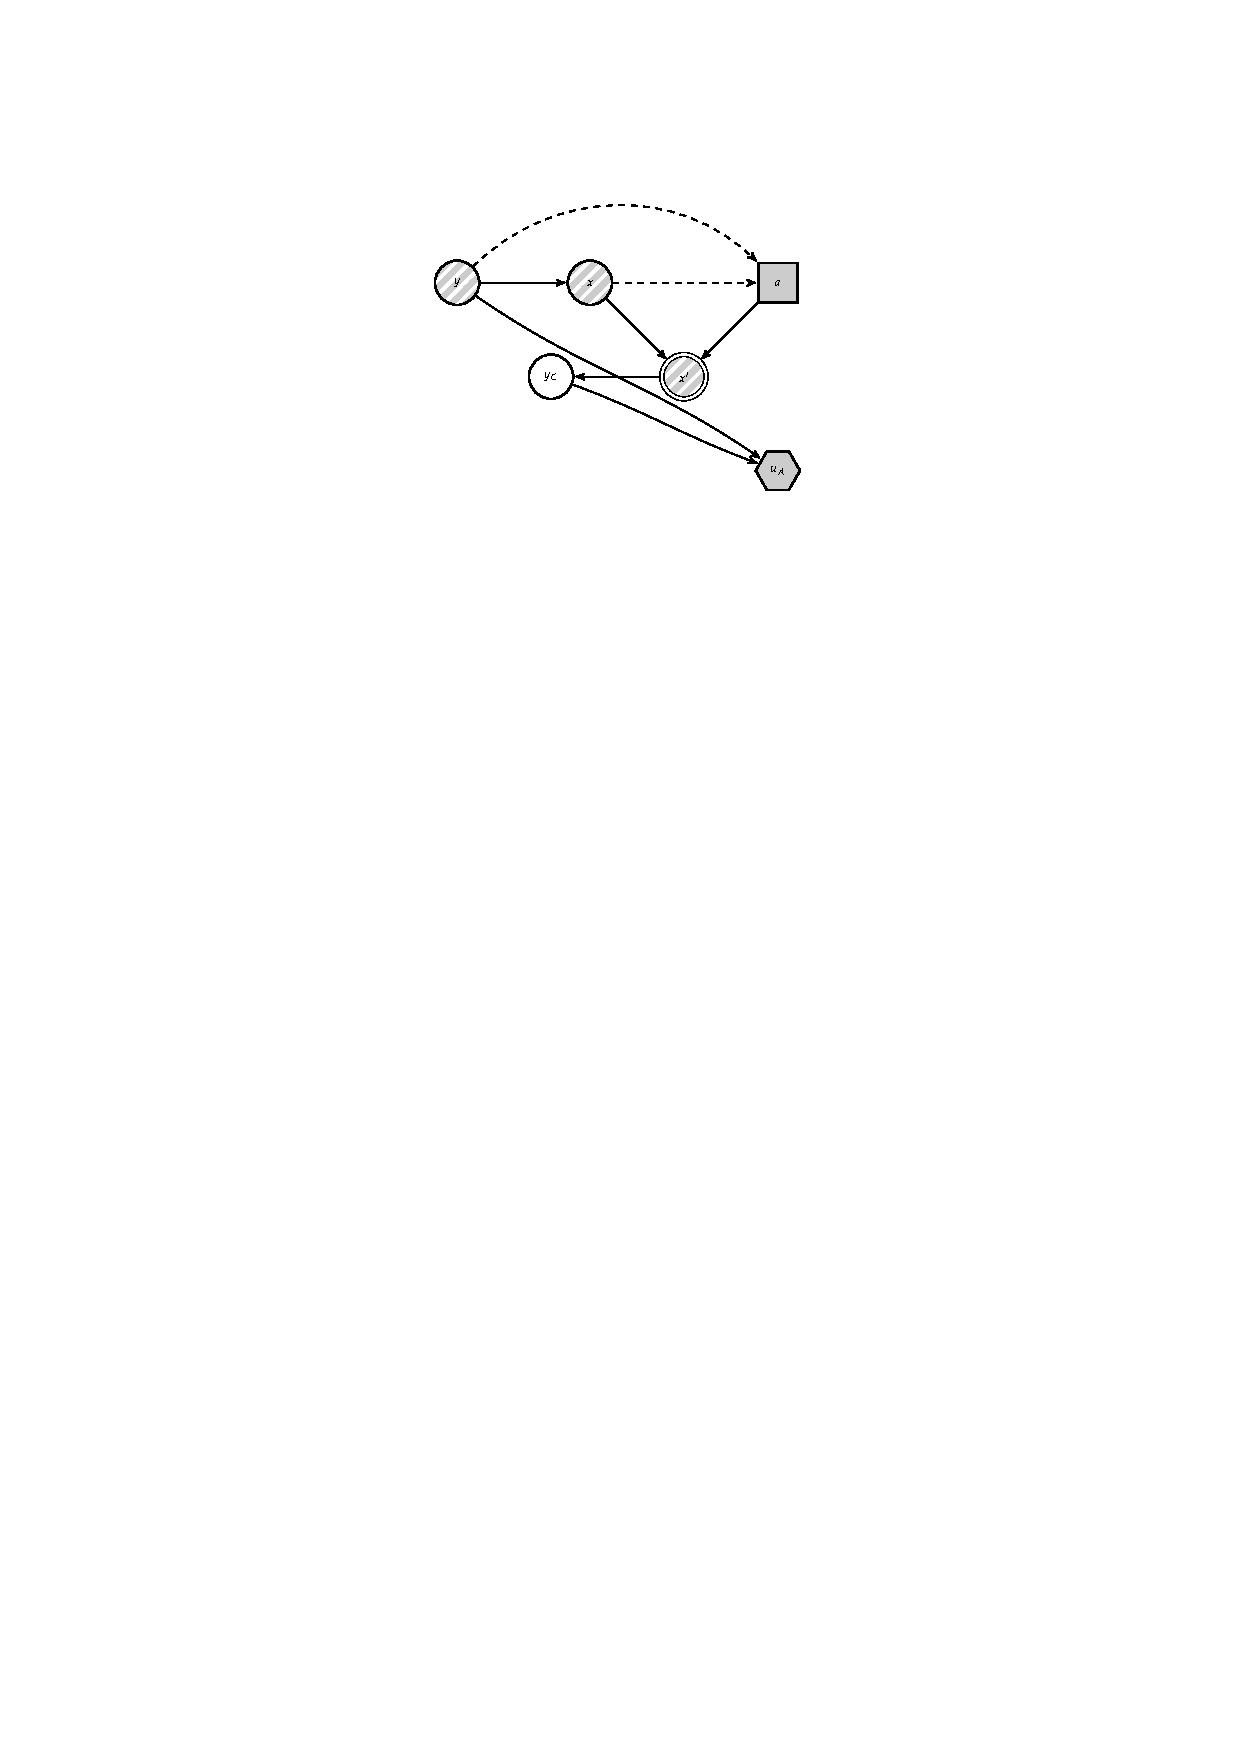
\includegraphics[scale=1]{figures/4.pdf}
\caption{Adversary problem.}\label{fig:adversaryProblem}\label{id}
\end{figure}
%It is natural, to assume that $p_A(x'|a,x)= I(x' = a(x))$.
To solve the problem, we need $p_A(y^*_c(x')|x')$, which models $A$'s beliefs about $C$'s decision when she observes $x'$.  Let
$p$ be the probability $p_A( y_c^* (a (x)) = y_1 | a (x) )$
that $A$ concedes to $C$ saying that the instance is malicious when she observes $x' = a(x)$. 
%
%
Since $A$ will have uncertainty about it, let us model its density using $f_A (p | x' = a(x) )$ with expectation $p_{x' = a(x)}^A $. Then, upon observing an instance $x$ of class $y_1$, $A$ would choose the data transformation maximising his expected utility:

%In addition, without loss of generality, we associate utility $0$ with the worst consequence for the attacker and $1$ with the best one, having the other consequences intermediate utilities  \parencite{french}. In the attacker's problem, his best consequence holds when the classifier accepts a malicious instance as benign (he has opportunities to continue with his operations) while the worst consequence appears when the defender stops a malicious one (he has wasted effort in a lost opportunity). Therefore, we assume  $U_A(y_1, y_1) \sim \delta_{0}$ and $U_A(y_2, y_1) \sim \delta_{1}$.
%
%In addition, without loss of generality, we assume that the attacker perceives positive utility $u_{21}$ when the defender misclassifies a bad instance classified as legitimate, and zero otherwise. 
%$$
%a^*(x, y )=\argmax_{a} \iint u_A(c(x'),y, a) \, \, p_A(x'|a, x) \, p_A(c|x') \,dx'\,dc ,
%$$
%or, equivalently,

\begin{eqnarray}\label{att_prob_n}
x'(x,y_1) &\equiv& a^*(x, y_1) = \argmax_{z} \int \bigg[ u_A( y_c^*(z) = y_1,y_1) \cdot p \nonumber\\
&+& u_A(y_c^*(z) = y_2, y_1) \cdot (1-p)\, \bigg] f _A (p | z = a(x) ) \dd p \nonumber \\
&=& \argmax_{z}
\left[ u_A(y_1,y_1) - u_A(y_2, y_1) \right] p_{z = a(x)}^A   +  u_A(y_2, y_1),
%\label{attackerprob}
\end{eqnarray}
%
where $u_A(y_i, y_j)$ is the attacker's utility when the defender classifies an instance of class $y_j$ as one of  class $y_i$. 

% Since we assume that $A$ does not change the data when $y=y_2$, that is $a^*(x, y_2) = x$, we only consider the case $y=y_1$. Then, $A$'s expected utility when he adopts attack $a$ and the instance is $(x,y_1)$ will be
% \begin{eqnarray*}
% \left[ u_A(y_1,y_1) - u_A(y_2, y_1) \right] p_{a(x)}^A  +  u_A(y_2, y_1).
% \end{eqnarray*}
        %which gets discretized to
%\begin{equation}
%  \scriptsize
%\argmax_{a} \int u_A(c(a(x)),+,a)p_A(+)p_A(x |+)p_A(c|a(x)) \,dc  + \int u_A(c(a(x))),-,a)p_A(-)p_A( x|-)p_A(c|a(x)) \,dc
%  \tag*{}
%\end{equation}

However, the classifier does not know the involved utilities $u_A$ and probabilities $ p_{z=a(x)} ^A $ from the adversary.
Let us model such uncertainty through a random utility function $U _A$ and a random expectation $ P_{z=a(x)}^A $. Then, we could solve for the random attack, optimising the random expected~utility
%
\begin{eqnarray*}
 X'(x,y_1) \equiv A^*(x, y_1) = \argmax_{z} \bigg(  \left[ U_A( y_1, y_1) - U_A( y_2, y_1) \right] P_{z=a(x)}^A   +    U_A( y_2, y_1) \bigg).
\end{eqnarray*}
%
We then use such distribution and make ({assuming that the set of attacks is discrete,
and similarly in the continuous case}) %Footnote was move here, please check.
$p_C(x'|x,y_1) =Pr(X'(x,y_1) = x')$ which was the missing
ingredient in 
problem \eqref{pis}. Observe that it could be the case that $Pr(X'(x,y_1)=x)>0$,
i.e., the attacker does not modify the~instance.

%Without loss of generality, we associate utility $0$ with the worst consequence and $1$ with the best one, having the other consequences intermediate utilities  \parencite{french}. In the attacker's problem, his best consequence holds when the classifier accepts a malicious instance as benign (he has opportunities to continue with his operations) while the worst consequence appears when the defender stops a malicious one (he has wasted effort in a lost opportunity). Therefore, we assume $U_A(y_1, y_1) \sim \delta_{0}$ and $U_A(y_2, y_1) \sim \delta_{1}$.
%
%The other consequences related with benign binaries are in between (and actually irrelevant). 
%    \begin{table}[H]
%    \centering
%    \begin{tabular}{cccc|}
%    \cline{3-4} & \multicolumn{1}{c}{} & \multicolumn{1}{|c|}{$y=M$} & %\multicolumn{1}{|c|}{$y=B$}\\
%    \cline{2-4}
%    \multicolumn{1}{c}{} & \multicolumn{1}{|c}{$y_{C}=M$} & %\multicolumn{1}{|c|}{$\delta_{0}$} & \multicolumn{1}{|c|}{$\alpha_{1}$}   \\
%    \cline{2-4}
%    & \multicolumn{1}{|c}{$y_{C}=B$} & \multicolumn{1}{|c|}{$\delta_{1}$} & %\multicolumn{1}{|c|}{$\alpha_{2}$} \\
%    \cline{2-4}
%    \end{tabular}
%    \caption{Alan's random utilities $U_A(y_c,y)$.}\label{tab:AlanRandomUti}
%    \end{table}
% Then, the Attacker's random optimal attack would be
%     \begin{equation}\label{eq:roa}
%     A^*(x,y_1) = \argmax_{a} \bigg[\Big( 0 - 1 \Big) P_{a(x)}^A + 1 \bigg] 
%          =  \argmin_{a}  P_{a(x)}^A .
%     \end{equation}

Now, without loss of generality, we can 
associate utility $0$ with the worst consequence and $1$ with the best one, having the other consequences intermediate utilities. In $A$'s problem, his best consequence holds when the classifier accepts a malicious instance as innocent (he has opportunities to continue with his operations) while the worst consequence appears when the defender stops an instance (he has wasted effort in a lost opportunity),
 other consequences being intermediate. Therefore, we 
adopt $U_A(y_1, y_1) \sim \delta_{0}$ and $U_A(y_2, y_1) \sim \delta_{1}$. Then, the Attacker's random optimal attack would be
\begin{equation}\label{random_att_prob_n}
X'(x,y_1) \equiv A^*(x, y_1) = \argmax_{z} \bigg[\Big( 0 - 1 \Big) P_{z=a(x)}^A + 1 \bigg] 
     =  \argmin_{z}  P_{z=a(x)}^A .
\end{equation}
Modelling $P^A _{z=a(x)}$ is more delicate. 
It entails strategic thinking and 
%s $C$ needs to understand his opponent's beliefs about what classification she will make when she observes $x'$. This 
could lead to a hierarchy of decision making problems, described in \textcite{rios2012adversarial} in a simpler context. 
A heuristic to assess it %to assess $P^A _{a(x)}$ may be
is based on using the probability $r=Pr _C (y_c^* (z) = y_1|z)$ that $C$ assigns to the instance received being malicious assuming that she observed $z$, with some uncertainty around it. 
As it is a probability, $r$ ranges in $[0,1]$ and we could make $P_{z=a(x)}^A \sim \beta e (\delta _1, \delta _2 )$, with mean $\delta _1 / (\delta _1 + \delta _ 2) = r$ and variance $ (\delta _1 \delta _2) / [(\delta _1 + \delta _2 )^2 (\delta _1 + \delta _2 + 1) ]=var $ as perceived. $var$ has to be tuned depending on the amount of knowledge $C$ has about $A$. Details on how to estimate $r$ are problem dependent.
%
% This leads to 
%  \begin{eqnarray}
%  \delta_{1}=\left( \frac{1-r}{\textit{var}} - \frac{1}{r} \right) r^2, \hspace{1cm}
%  \delta_{2}=\delta_{1}\bigg(\frac{1}{r}-1\bigg) . \label{deltas}
%  \end{eqnarray}
% Conceptually, given the observed $x'$, we could consider all attacks leading to it, differentiating between instances with original label $y_1$ and those with original label $y_2$; compute the probabilities of observing the malicious ones and adding them to obtain $p_1$ and perform the same process with innocent instances to obtain $p_2$; and, finally make $r=p_1 / (p_1+p_2)$.

In general, to approximate $p_C(x'|x,y_1)$ we use
Monte Carlo (MC) simulation drawing $K$ samples $\bigl(P_{z} ^{A,k} \bigr)$, $k = 1,\dots,K\, $
from  $P_{z} ^{A}$, finding
%
$ X'_k (x, y_1)=\argmin_{z}  P_{z} ^{A,k}
$ %
  and estimating $p_C(x'|x,y_1)$ using the proportion of times in which the result of the random optimal attack coincides with the instance actually observed by the defender:
\begin{eqnarray}
\widehat{p}_C ( x'\,|\,x, y_1) =  \frac {\# \{X'(x, y_1) =  x'\}} {K}. \label{mc_estimate}
\end{eqnarray}
It is easy to prove, using arguments in \textcite{10.5555/3172929}, that \eqref{mc_estimate} converges almost surely to $p_C (x'|x,y_1)$.
{In this, and other MC approximations considered, 
recall that the sample sizes  are essentially dictated by the required
    precision. 
    Based on the Central Limit Theorem \parencite{Chung},
    MC sums approximate integrals with probabilistic bounds
    of the order $\sqrt{\frac{var}{N}}$ where $N$ is the MC sum size.
    To obtain a variance estimate, we run a few iterations and estimate 
    the variance, then choose the  required size based on such bounds.}%Footnote was move here, please check.

Once we have 
an  approach to estimate the required probabilities, 
%as in \eqref{mc_estimate}, %which entails the availability of a routine to generate from the random utility function, as in the Appendix, 
we implement the scheme described through
Algorithm \ref{alg:uno}, which reflects an initial training 
phase to estimate the classifier and an operational phase
which performs the above once a (possibly perturbated)
instance $x'$ is received by the classifier.

\begin{algorithm}[ht] % 
\caption{General adversarial risk analysis (ARA) procedure for AC. Generative}  
\label{alg:uno}
\begin{algorithmic}[1]
\State {\bf Input:} Training data $\mathcal{D}$, test instance $x'$.
\State {\bf Output:} A classification decision $y_c^*(x')$.
\Train
\State Train a generative classifier to estimate $p_C(y)$ and $p_C(x|y)$
%\State (the training set is not tainted).
\EndTrain
\Operation
\State Read $x'$.
\State Estimate $p_C(x' |x,y_1)$ for all $x \in \mathcal{X}'$.
\State Solve
\begin{eqnarray*}
y_c^*(x') &=& \argmax_{y_C} \bigg[ u_C(y_C, y_1) \widehat{p}_C(y_1) \sum_{x\in \mathcal{X}'} \widehat{p}_C(x' |x,y_1) \widehat{p}_C(x|y_1) 
\\ &+& u_C(y_C, y_2) \widehat{p}_C(x'|y_2)\widehat{p}_C(y_2)\bigg].
\end{eqnarray*}
\State Output $y_c^*(x')$.
\EndOperation
\end{algorithmic}
\end{algorithm}




\section{Scalable Adversarial Classifiers}\label{sec:scalable}
%
The approach in Section \ref{sec:ac_acra} performs all relevant inference about the adversary during operations, and is only suitable for generative models, such as Naive Bayes. This could be too expensive computationally, especially in applications that require fast predictions
based on large scale deep models as motivated by the following image
processing problem.

%can be too expensive computationally in large scale problems, making its application unfeasible. As a motivation, consider an image processing problem dealt with a deep learning model.

%%%%%%%%%%%%%%%%%%%%%%%%%%%%%%%%%%%%%
\paragraph{Attacks to neural-based classifiers.}
Section \ref{sec:other_AC} discussed adversarial examples.  This kind of attack may harm intensely neural
network performance, such as that used in image classification tasks \parencite{szegedy2013intriguin}. It has been shown that simple one-pixel attacks can seriously affect performance \parencite{su2019one}.
As an example, we continue the discussion started in the introduction of this thesis, in Section \ref{sec:chall2}. Consider 
a relatively simple deep neural network (a multilayer perceptron model) \parencite{10.5555/3086952}, trained to predict the handwritten digits in the MNIST dataset \parencite{MNIST}. In particular, we used a 2 layer feed-forward neural network with relu activations and a final softmax layer to compute the predictions over the 10 classes. This requires simple extensions from binary to multi-class classification. This network accurately predicts 99\% of the digits. Figure \ref{fig:10samples} provides ten MNIST original 
samples (top row) and the corresponding images (bottom row) perturbed through FGSM,
which are misclassified. For example, the original 0 
(first column) is classified
as such; however, the perturbed one
is not classified as a 0 (more specifically, as an 8) even if it looks as such to the human~eye.%Footnote was move here, please check.

% with a relatively simple deep neural network (a multilayer perceptron model) \parencite{10.5555/3086952}, we accurately predict 99\% of the handwritten digits in the MNIST data set \parencite{MNIST}.
% {\bf In particular, we used a 2 layer feed-forward neural network with relu activations and a final softmax layer to compute the predictions over the 10 classes}.  
% \footnote{{\bf This requires simple extensions from binary classification to multiple
% class calssification.}}
% Figure \ref{fig:10samples} provides ten MNIST original 
% samples (top row) and the corresponding images (bottom row) perturbed through FGSM,
% which are misclassified. For example, the original 0 
% (first column) is classified
% as such; however the perturbed one
% is not classified as a 0 (more specifically, as an 8) even if it looks as such to the human eye.

\begin{figure}[H]
\centering
  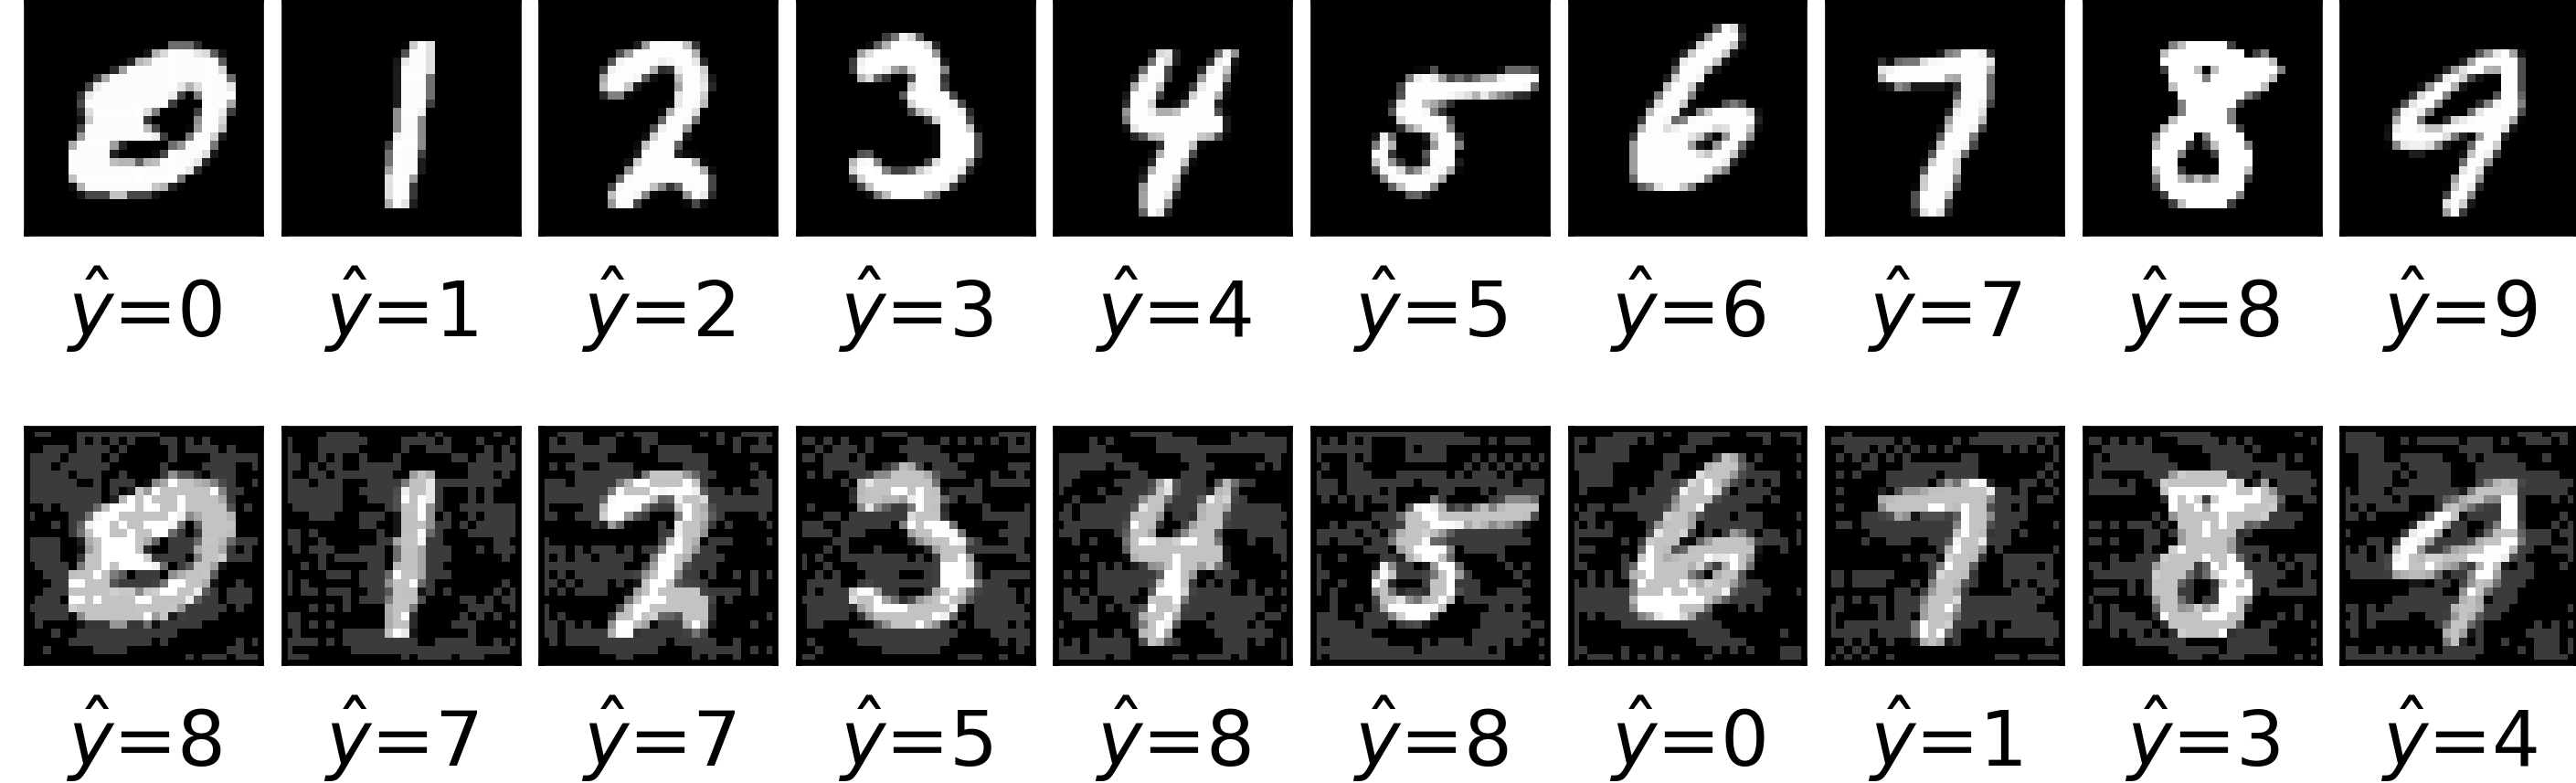
\includegraphics[scale=1.]{figures/10samples.png}
  \caption{Ten MNIST examples (top) and their perturbations (bottom). Predicted class shown for each~example.}
  \label{fig:10samples}
\end{figure}
Globally, accuracy gets reduced to around 50\% (see Figure \ref{fig:comparison_mnist}a, curve NONE far right). This suggests a very important performance degradation due to the attack. Section \ref{sec:exp_scalabl} continues this example to evaluate the robustification procedure we introduce in Section  \ref{sec:uncs}. \\

The computational difficulties entailed by 
the approach in Section \ref{sec:ac_acra} stem from the following issue:
iterating over the set $\mathcal{X}'$ of potentially
originating instances.  
 If no assumptions about attacks are made, this set grows rapidly.
 For instance, in the spam detection example in Section \ref{sec:att_class}, 
 let $n$ be the number of words in the dictionary considered by
 $C$ to undertake the classification (54 in our spam case). If 
 we assume that the attacker modifies at most one word,
 the size of $\mathcal{X}'$ is $\mathcal{O}(n)$; if he modifies at most two words, it is $\mathcal{O}(n^2)$, $\dots$, and 
 if he modifies at most $n$ words, 
 the number of possible adversarial manipulations (and thus the size of $\mathcal{X}'$) is $2^n$.
 
   Even more extremely, in the 
 image processing example we would have to deal with
 very high-dimensional data (the MNIST images above consist of $28 \times 28$ pixels, each taking 256 possible values depending on the gray level). 
 This deems any enumeration over the set $\mathcal{X}'$ totally unfeasible. In order to tackle this issue,
 constraints over the attacks could be adopted, for example 
 based on distances.
 
  
 Therefore, as the key adversary modelling steps are taken during operations,
 the approach could be inefficient in applications requiring fast predictions.
  
 
 
 %%%%%%%%%%%%%%%%%%%%%%%%%%%%%%%%%%
 \subsection{Protecting Differentiable Classifiers}\label{sec:uncs}
 
Alternatively, learning about the adversary 
could be undertaken during the training phase as now 
presented. This provides faster predictions during operations and avoids the expensive step of sampling from $p_C(x \vert x')$.
A relatively weak assumption is made to achieve this: 
the model is probabilistic and can be differentiable in the $\beta$ parameters.
By this we understand classifiers with structural form 
$p_C(y|\beta,x)$ differentiable in $\beta$. 
A specially relevant form %lopments (and in classification applications at large) are models based on a parameterized function $f_\beta : \mathbb{R}^d \rightarrow \mathbb{R}^k,$ in which the prediction
is 
%
\begin{eqnarray}\label{TGF}
p(y|\beta, x) = \mbox{softmax} (f_\beta (x))[y], & \text{where} & \mbox{softmax}(x)[j] = \frac{\exp{x_j}}{\sum_{i=1}^k \exp{x_i} }. 
\end{eqnarray}
%
This covers a large class of models. For example,
if $f_\beta$ is linear in inputs, %, $f_\beta (x) = \beta' x$, 
we recover multinomial regression 
\parencite{mccullagh1989generalized}; if we take $f_\beta$ to be a sequence of linear transformations alternating non-linear activation functions, such as Rectified Linear Units (ReLU), we obtain a feed-forward neural network \parencite{10.5555/3086952}. 
These models have the benefit of being amenable to training using \emph{stochastic gradient descent} (SGD) \parencite{bottou2010large},
or any of its recent variants, such as Adam \parencite{kingma2014adam}, 
allowing for scaling to both wide and tall datasets. Then, from SGD we can obtain the posterior distribution of the model by adding a suitable noise term as in SG-MCMC samplers like stochastic gradient Langevin Dynamics (SGLD) \parencite{welling2011bayesian} or accelerated variants such as the ones introduced in chapter 2 of this thesis.

 %To avoid the bottleneck of sampling 
 %from $p_C(x|x')$,
 We require  
 only sampling attacked instances from $p_C(x'|x)$, an attacker model. Depending on the type of data, this model can
 come through a discrete optimisation problem
 (as in the attacks of Section \ref{sec:att_class}) or a continuous optimisation problem
 (in which we typically resort to gradient information to obtain the most harmful perturbation 
 as in FGSM).
 These attacks require white-box access to the defender model, 
which, as mentioned, is usually unrealistic in security.
With continuous data, adversarial perturbations $x'$ 
are typically computed through the optimization problem
$$
x'= \arg\min_{x' \in B(x)} \log p(y|x',\beta),
$$ 
where $B(x)$ is some neighborhood of $x$ 
over which the attacker has influence on.
Exact solution of this problem is intractable in high-dimensional data.
Thus, attacks in the literature resort to approximations using gradient information. One of the most popular ones is FGSM,  
given by $x' = x -\epsilon\, \mbox{sign} \nabla_x \log p(y|x,\beta)$ where $\epsilon$ is a step size 
 reflecting attack intensity. Other attack examples 
include the Projected Gradient Descent (PGD) \parencite{madry2018towards} or the
\textcite{carlini2017towards} attack. 
These assume that the attacker has full knowledge of the target model,
which is unrealistic in many scenarios. 
AT using FGSM would correspond to sampling from a Dirac delta distribution centered at the FGSM update, %$\left( x -\epsilon \nabla_x \log p(y|x,\beta)\right)$, 
that is, $p(x'|x) = \delta (x' - (x -\epsilon \mbox{ sign} \nabla_x \log p(y|x,\beta)))$. 

More realistically, based on ARA, we 
apportion two sources of uncertainty.
%y,
%adding realism to AT.  
%e extend thus AT by introducing two sources of uncertainty.

%In our framework, AT using FGSM would correspond to sampling from a Dirac delta distribution centered at $\left( x -\epsilon \nabla_x \log p(y|x,\beta)\right)$, that is, $p(x'|x) \sim \delta (x' - (x -\epsilon \mbox{sign} \nabla_x \log p(y|x,\beta)))$. More realistically, we introduce two sources of uncertainty.

%%%%%%%%%%%%%%%%%%%%%%%%%%%%%%%%%%%%%%%%%%%%%%%%%%%%%%%%%%%%%

\paragraph{Defender uncertainty over the attacker model $p_C(x'|x)$.}

 The attacker modifies data in the operation phase.
 The defender has access only to training data $\mathcal{D}$; therefore, 
 she will have to simulate attacker's actions using such training set. Now, uncertainty can also come from the adversarial perturbation chosen. If the model is also differentiable wrt the input $x$ (as 
 with continuous data such as images or audio), instead of computing a single, optimal and deterministic perturbation, as in AT, we use SGLD to sample adversarial examples from regions of high adversarial loss, adding a noise term to generate uncertainty. Thus, we employ iterates of the form
\begin{equation}\label{eq:unc_attack}
x_{t+1} = x_t -\epsilon\, \mbox{sign} \nabla_x \log p_C(y|x_t,\beta) + \mathcal{N}(0, 2\epsilon),
\end{equation}
for $t=1,\ldots,T$, where $\epsilon$ is a step size. We can also consider uncertainty over the hyperparameters $\epsilon$ (say, from a rescaled Beta
distribution, since it is unreasonable to consider too high or too low learning rates) and the number $T$ of iterations (say, from a Poisson distribution). In addition, we can consider mixtures of different attacks, for instance by sampling a Bernoulli random variable and, then, choosing the gradient corresponding to either FGSM or another 
attack such as Carlini and Wagner's. 




%In addition, we can consider mixtures of different attacks, for instance by sampling a Bernoulli random variable and then choosing the gradient corresponding to either FGSM or the \parencite{carlini2017towards} attack.
%%%%%%%%%%%%%%%%%%%%
\paragraph{Attacker uncertainty over the defender model $p_C(y|x,\beta)$.}

It is reasonable to assume that the specific model architecture and parameters %$p_C(y|x,\hat{\beta})$ 
are unknown by the attacker. %, for a fixed set of weights $\hat{\beta}$.
To reflect his uncertainty, he will instead perform attacks over
a model $p_C(y|x,\beta)$ with uncertainty  
over the values of the model parameters $\beta$, with continuous
support. 
This can be implemented through scalable Bayesian approaches
in deep models: the defended model is trained using SGLD, obtaining posterior samples via the iteration
\begin{equation}\label{eq:unc_model}
\beta_{t+1} = \beta_t + \eta \nabla_\beta (\log p(y|x, \beta) + \log p(\beta)) + \mathcal{N}(0, 2\eta I),
\end{equation}
with $\eta$ a learning rate, and $x$ sampled either from
the set $\mathcal{D}$ (untainted) or using an attacker model as in the previous point. We sample maintaining
a proportion 1:1 of clean and attacked data.  To see that this sampling method actually samples
from the  posterior $p(\beta| \mathcal{D})$,
where 
$\mathcal{D}$ designates a mixture of the clear and attacked dataset, just note that the Langevin SG-MCMC sampler for the posterior can be written as
$$
\beta_{t+1} = \beta_{t} + \eta \nabla \log p(\beta | \mathcal{D})  + \mathcal{N}(0, 2\eta I).
$$
Noting that $\log p(\beta | \mathcal{D}) = \log p(\mathcal{D} | \beta ) + \log p(\beta) - \log p(\mathcal{D})$ and taking gradients wrt to $\beta$ we have that $\nabla \log p(\beta | \mathcal{D}) = \nabla \log p(\mathcal{D} | \beta ) + \nabla \log p(\beta)$. An unbiased estimator of the gradient is obtained by replacing the whole dataset with just a single sample, or a minibatch, leading to the sampler in Eq. (\ref{eq:unc_model})
with $x \sim \mathcal{D}$. \\


%, as prescribed by the ARA framework.

%\begin{algorithm}[tb] % 
%\caption{Large scale attack simulation}  
%\label{alg:large_attack}
%\begin{algorithmic}[1]
%\State {\bf Input:} Defender model $p(y|x,\beta)$, a set of particles $\lbrace \beta_i \rbrace_{i=1}^K$ and attacker model $p(x'|x)$. 
%\State {\bf Output:} A set of adversarial examples $\{x_i\}_{i=1}^{K}$ from the attacker model. 
%\Operation
%\State Sample initial set of particles from prior: $\mathbf{z}_1^0, \mathbf{z}_2^0, \ldots \mathbf{z}_K^0 \sim \pi(\mathbf{z})$.
%\State sample $T \sim p(T)$
%\State sample $\epsilon \sim p(\epsilon)$
%\For{each attack iteration $t$ from $1$ to $T$}
%\State $x_{i,t+1} = x_{i,t}  -\epsilon\, \mbox{sign} \nabla_x \log p(y|x_t,\beta)  + \mathcal{N}(0, 2\epsilon)$
%\EndFor
%\State Output $x_i = x_{i,T}$
%\EndOperation
%\end{algorithmic}
%\end{algorithm}


The previous approaches incorporate some uncertainty about the attacker's elements to sample from $p_C(x' \vert x)$. A full ARA sampling from this distribution could be performed as well. 
Algorithm \ref{alg:large_ara} describes how to generate samples incorporating both types of uncertainty previously described. On the whole, it uses the first source to generate perturbations to robustly train the defender's model based on the second source. 


\begin{algorithm}[!ht] % 
\caption{Large scale ARA-robust training for AC}  
\label{alg:large_ara}
\begin{algorithmic}[1]
\State {\bf Input:} Defender model $p_C(y|x,\beta)$, attacker model $p_C(x'|x)$. 
\State {\bf Output:} A set of $k$ particles $\{\beta_i\}_{i=1}^{K}$  approximating the posterior distribution of the defender model learnt using ARA training.  
%\State Sample initial set of particles from prior: $\mathbf{z}_1^0, \mathbf{z}_2^0, \ldots \mathbf{z}_K^0 \sim \pi(\mathbf{z})$.
\For{$t=1$ to $T$}
\State Sample $x_1, \ldots,  x_K \sim p_C(x' | x)$ with 
(\ref{eq:unc_attack}).
\State $\beta_{i,t+1} = \beta_{i,t} + \eta \nabla_\beta (\log p_C(y|x, \beta) + \log p(\beta)) + \mathcal{N}(0, 2\eta )$ for each $i$ (SGLD)
\EndFor
\State Output $(\beta_{1,T},...,\beta_{K,T}))$
\end{algorithmic}
\end{algorithm}

Very importantly, its outcome tends to be more robust  than
the one we could achieve with just AT protection, since we incorporate some level of adversarial uncertainty. In the end, we collect $K$ posterior samples, $\lbrace \beta_k \rbrace_{k=1}^K$, and compute predictive probabilities for a new sample $x$ via marginalisation
through
$p_C(y|x) = \dfrac{1}{K} \sum_{k=1}^K p_C(y|x, \beta_k)$,
using the previous predictive probability to robustly classify the
received instance.

%Section \ref{sec:exp_scalable} performs several experiments applying the previous scalable approaches to the spam detection task from Section \ref{sec:att_class}. To see a similar framework applied to image classification tasks, the reader can check \parencite{gallego2020protecting}.

 




%%%%%%%%%%%%%%%%%%%%%%%%%%%%%%%%%%%%%%%%%%%%%%%%%%%%
\section{Case Studies}
\label{sec:conEx}

We use the spam classification dataset from Section \ref{sec:att_class} 
and the MNIST dataset to illustrate the methods in Section \ref{sec:scalable}. As shown in Section \ref{sec:att_class}, simple attacks such as good/bad word insertions are sufficient to
critically affect the performance of spam detection algorithms. The small perturbations from Section \ref{sec:scalable} prove that unprotected image classification systems can easily be fooled by an adversary. 
%We first test the performance of the ARA approach to AC in Section \ref{acra:disc}, as a defence mechanism against attacks that modify at most 2 words. For the classifier, we use a 0-1 utility model.
%We test our results using the dataset in Section \ref{sec:att_class}.


%%%%%%%%%%%%%%%%%%%%%%%%%%%%%%%%%
\subsection{Robustified Classifiers in Spam Detection Problems}\label{sec:exp_scalable}

For the first batch of experiments, we use the same classifiers as in
 Section \ref{sec:scalable}. As a dataset, we use again the UCI Spam Data Set from that section. Once the models to be defended are trained, we perform attacks
 %as underlying classification algorithms we deploy a two layer neural network, a random forest, a support vector machine and a logistic regression with L1 regularization. \footnote{This last one is equivalent to performing maximum a posteriori estimation in a logistic regression model with a Laplace prior \parencite{park2008bayesian}.}
 % Mean and standard deviations of accuracies are estimated via repeated %hold-out validation over ten repetitions \parencite{kim2009estimating}.
%The accuracy of this approach on clean test data is $0.68 \pm 0.01$. 
% Attacker parameters
%To compare AB-ACRA with the raw classifiers on tampered data,
over the instances in the test set, solving 
problem \eqref{random_att_prob_n} for each test spam email, removing the uncertainty that is not present from the adversary's point of view. 
We next evaluate the scalable approach in Section \ref{sec:scalable} under the two differentiable models
among the previous ones: logistic regression and neural network (with two hidden layers). %We choose these two models from the complete set displayed in Table \ref{tab:acra_vs_raw} since
As required, both models can be trained using SGD plus noise methods to obtain uncertainty estimates from the posterior as in (\ref{eq:unc_model}). %Again, attackers may modify up to two words. 
Next, we attack the clean test set using the procedure 
in Section \ref{sec:att_class} and evaluate the performance of 
our robustification proposal. % (with and without adding uncertainties from Section \ref{sec:uncs}). 
Since we are dealing with discrete attacks, we cannot use the uncertainty over attacks as in (\ref{eq:unc_attack}) and just resort to adding the attacker's uncertainty over the defender model as in (\ref{eq:unc_model}). To perform classification with this model, we evaluate the Bayesian predictive distribution using $5$ posterior samples obtained after SGLD iterations.
Results are in Table \ref{tab:rob_exps} which include as 
entries:
Acc.\ Unt. (accuracy over untainted data); 
Acc.\ Tai. (it.\ over tainted data);
%Acc.\ Rob.\ NoU., the accuracy over tainted data after robustification, without adding uncertainties (the  vanilla AT in Section \ref{sec:other_AC});
Acc.\ Rob.\ Taint.\ (it.\ over tainted data after
our robustification adding uncertainties).
Note that the first two columns do not coincide with those
in Table \ref{tab:cleanVSattack}, as we have changed 
the optimisers to variants of SGD to be amenable to  
the robustified procedure in Section \ref{sec:uncs}.

%& Acc. Rob. NoU.
%$0.944 \pm 0.005$ &
%$0.941 \pm 0.006$&

\begin{table}[H]
\caption{Accuracy 
	of two classifiers on clean
	(untainted), and attacked (tainted) data, with and without robustification.}
	\centering
	\begin{tabular}{cccc}
		\toprule
		\textbf{Classifier }& \textbf{Acc. Unt.} & \textbf{Acc. Tai.}  & \textbf{Acc. Rob. Taint.} \\
		\midrule
		Logistic Reg.  & $0.931 \pm 0.007$    & $0.705 \pm 0.009$ &    $0.946 \pm 0.003$  \\  
		Neural Net  &      $0.937 \pm 0.005$     &     $0.636 \pm 0.009$    &     $0.960 \pm 0.002$  \\

		\bottomrule
	\end{tabular}%
	\label{tab:rob_exps}%
\end{table}%

Observe that the proposed robustification process
 indeed protects differentiable classifiers, 
 recovering from the degraded performance under attacked
 data. Moreover, in this example, the robustified classifiers
  achieve even higher accuracies than those attained by the original classifier over clean data. This is likely due to the fact that the presence of an adversary has a regularizing effect, being able to improve the original accuracy of the base algorithm and making it more robust. %For the simple linear classifier, average accuracies remain similar %whether we use a single model (no uncertainty) or a Bayesian ensemble %(uncertainty), yet the later one has a smaller standard deviation, %consistent with the fact that ensembling helps in maintaining stability in %performance along different experiment runs. Regarding the neural %classifier, observe that the Bayesian variant achieves significantly %higher accuracy.} 


\subsection{Robustified Classifiers in Image Classification Problems}\label{sec:exp_scalabl}


Next, we show the performance of the scalable approach continuing with the digit recognition example from Section \ref{sec:scalable}. This batch of experiments aims to show that the ARA-inspired defence  can also scale to high-dimensional feature spaces and multiclass problems. The 
network architecture is shown in Section \ref{sec:scalable}. It is trained using SGD with momentum ($0.5$) for 5 epochs, with learning rate of $0.01$ and batch size of 32. The training set includes 50,000 digit images, and we report results over a 10,000 digit test set. As for uncertainties from Section \ref{sec:uncs}, we use both kinds. 


\begin{figure}[!htb]
\begin{center}
\minipage{0.45\textwidth}
\hspace{-0.5em}
  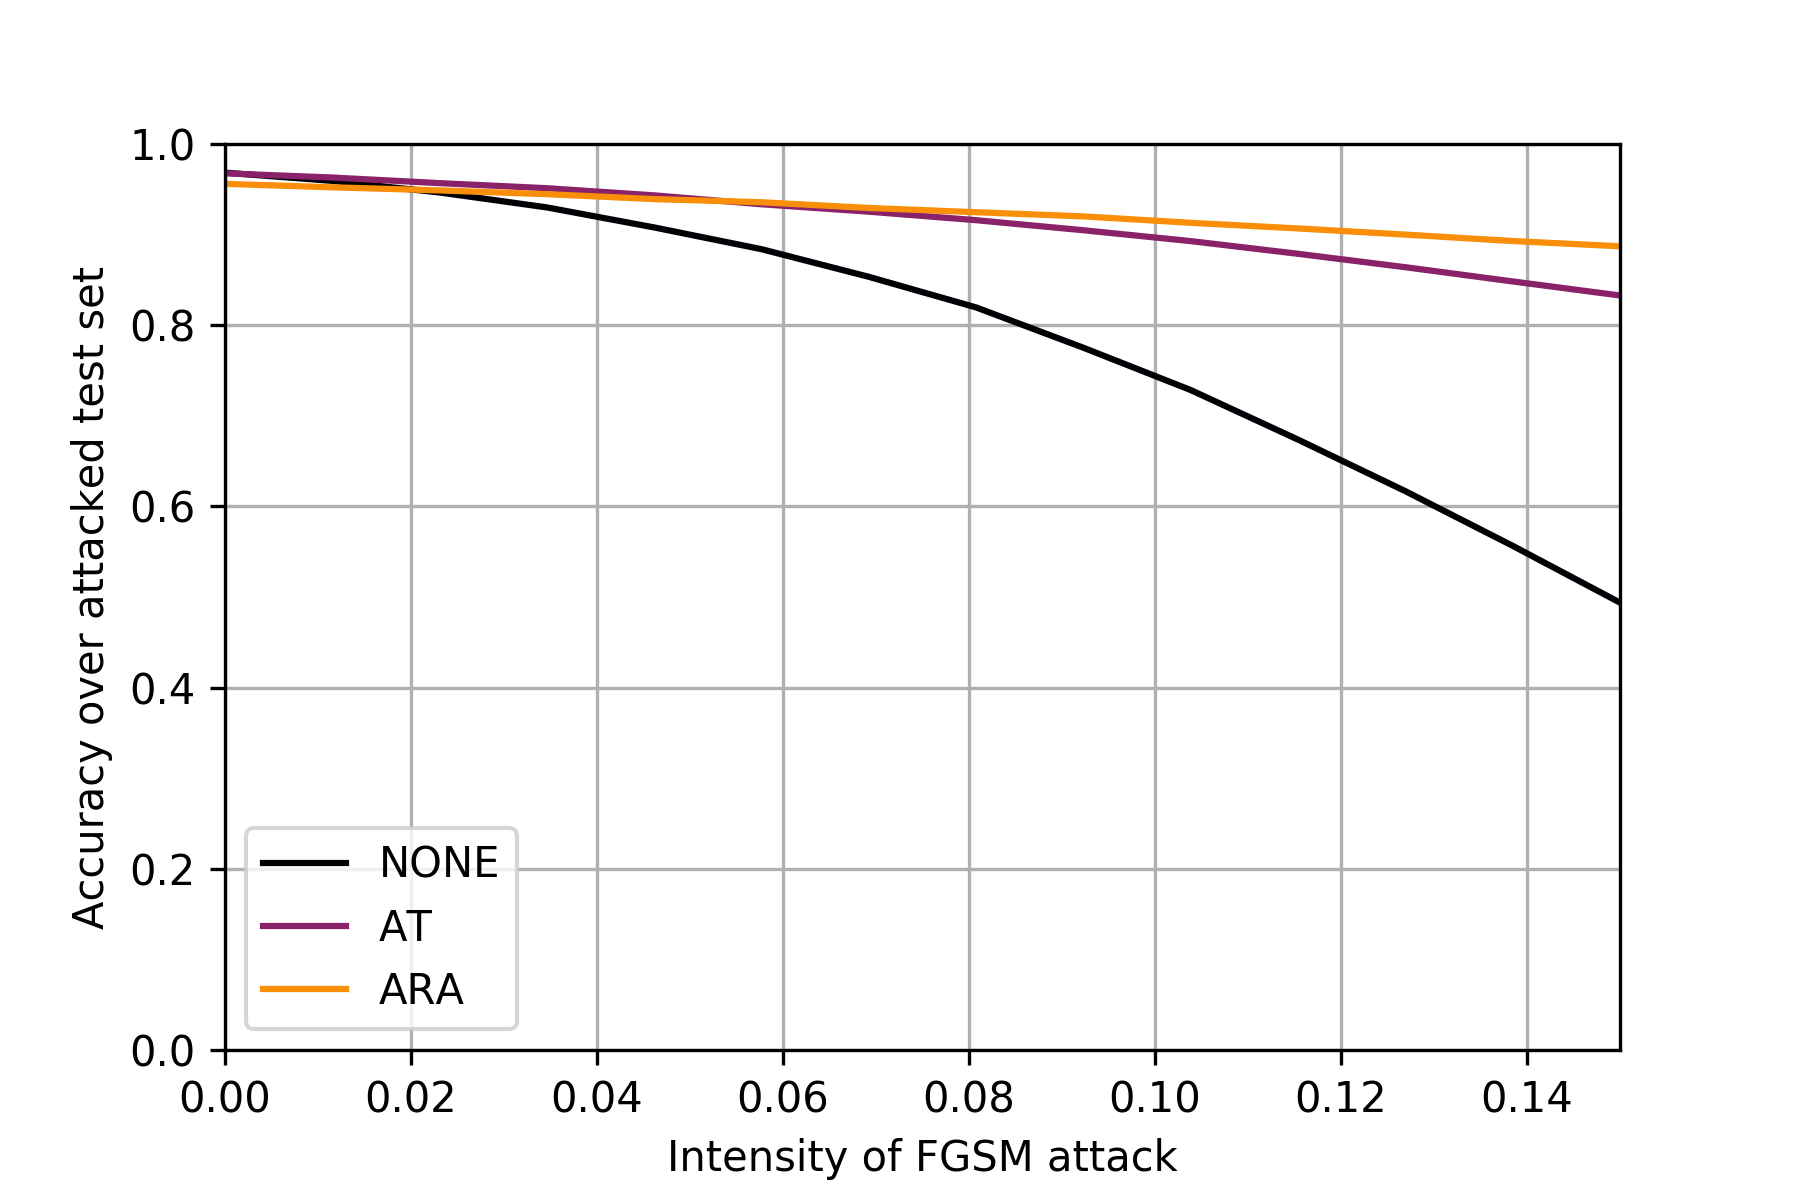
\includegraphics[width=\textwidth]{figures/comparison_mnist_fgsm.png}
   \caption{FGSM attack.}
\endminipage\hfill
\minipage{0.45\textwidth}
  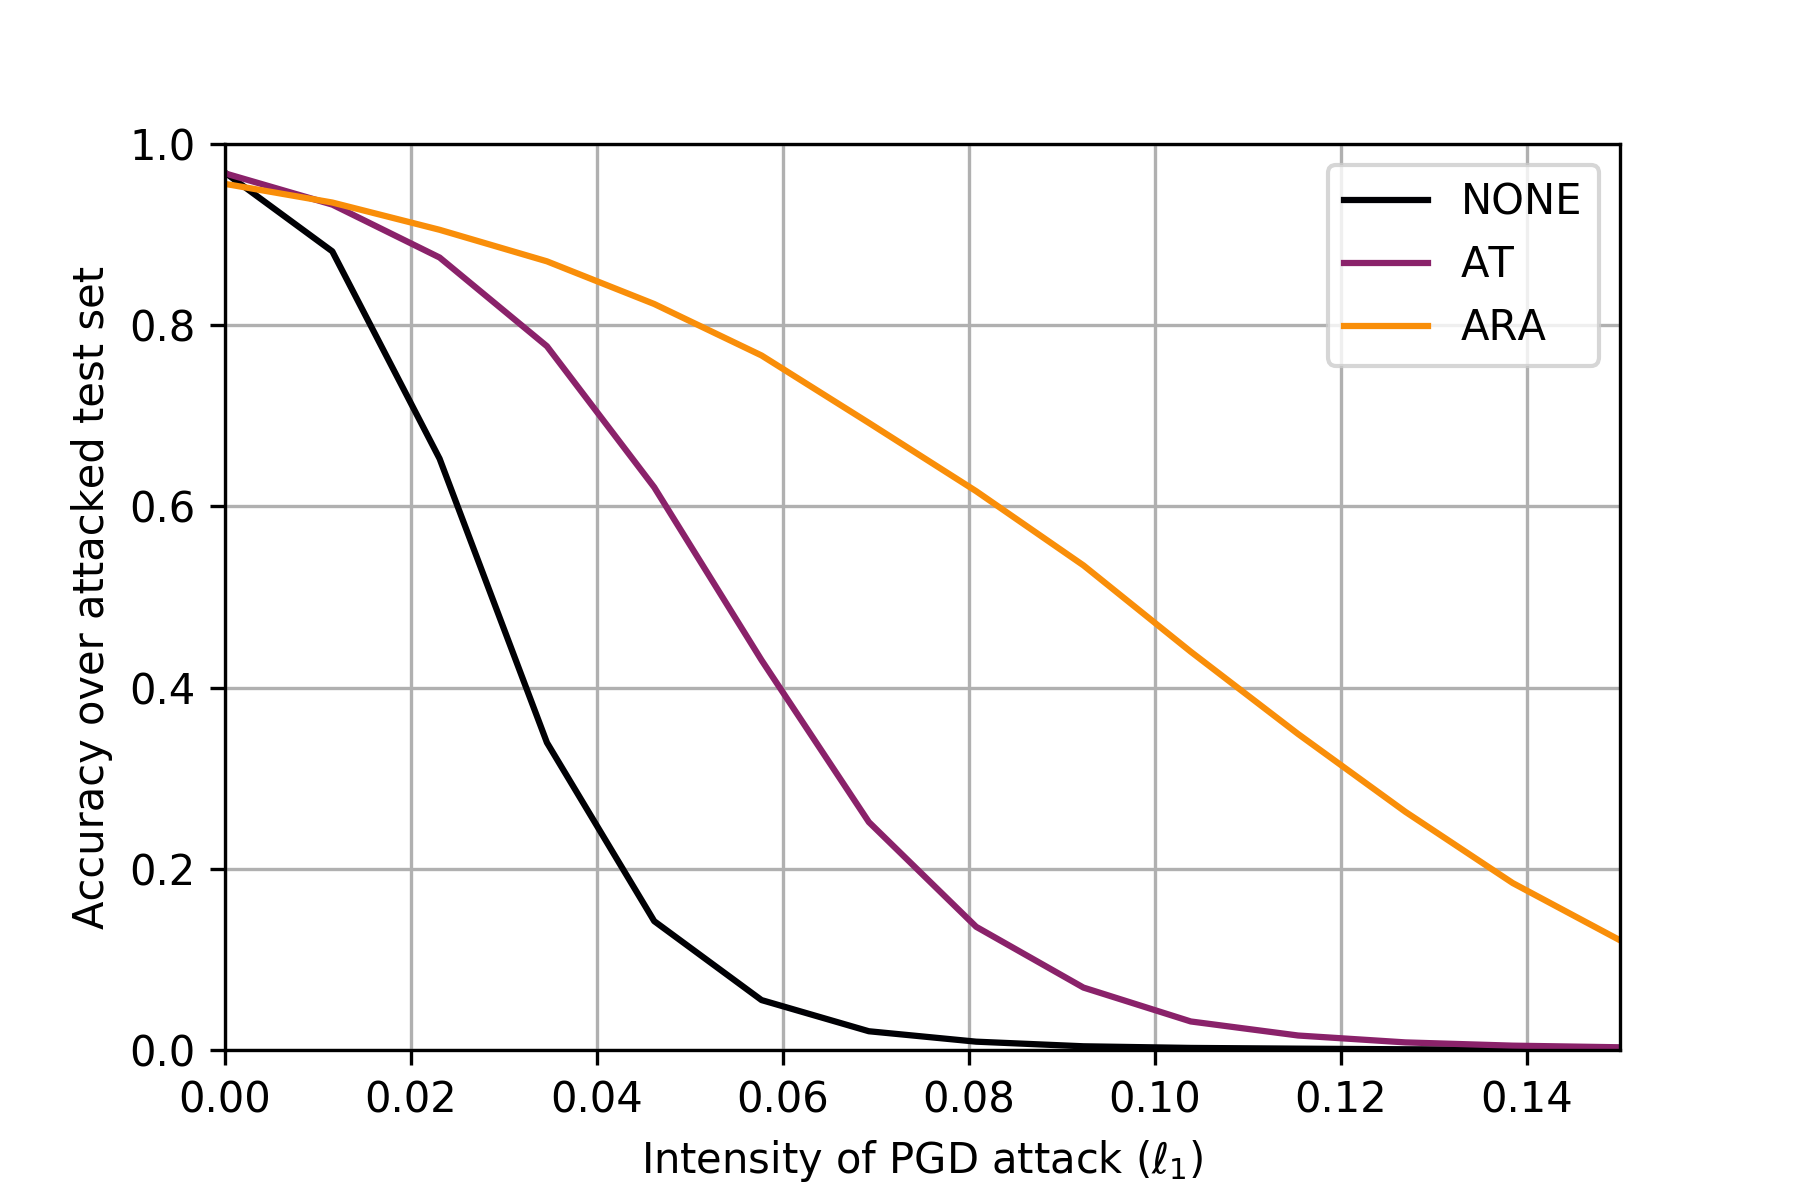
\includegraphics[width=\textwidth]{figures/comparison_mnist_pgdl1.png}
   \caption{PGD attack under $\ell_1$ norm.}
\endminipage
\end{center}
\caption{Robustness of a deep network for MNIST under three defence mechanisms 
(none, AT, ARA). (a) depicts the security evaluation curves under the FGSM attack. (b) depicts the security evaluation curves under the PGD attack.}\label{fig:comparison_mnist}
\end{figure}

\iffalse

\begin{figure}[!htb]
    \centering
    \begin{subfigure}[b]{0.45\textwidth}
        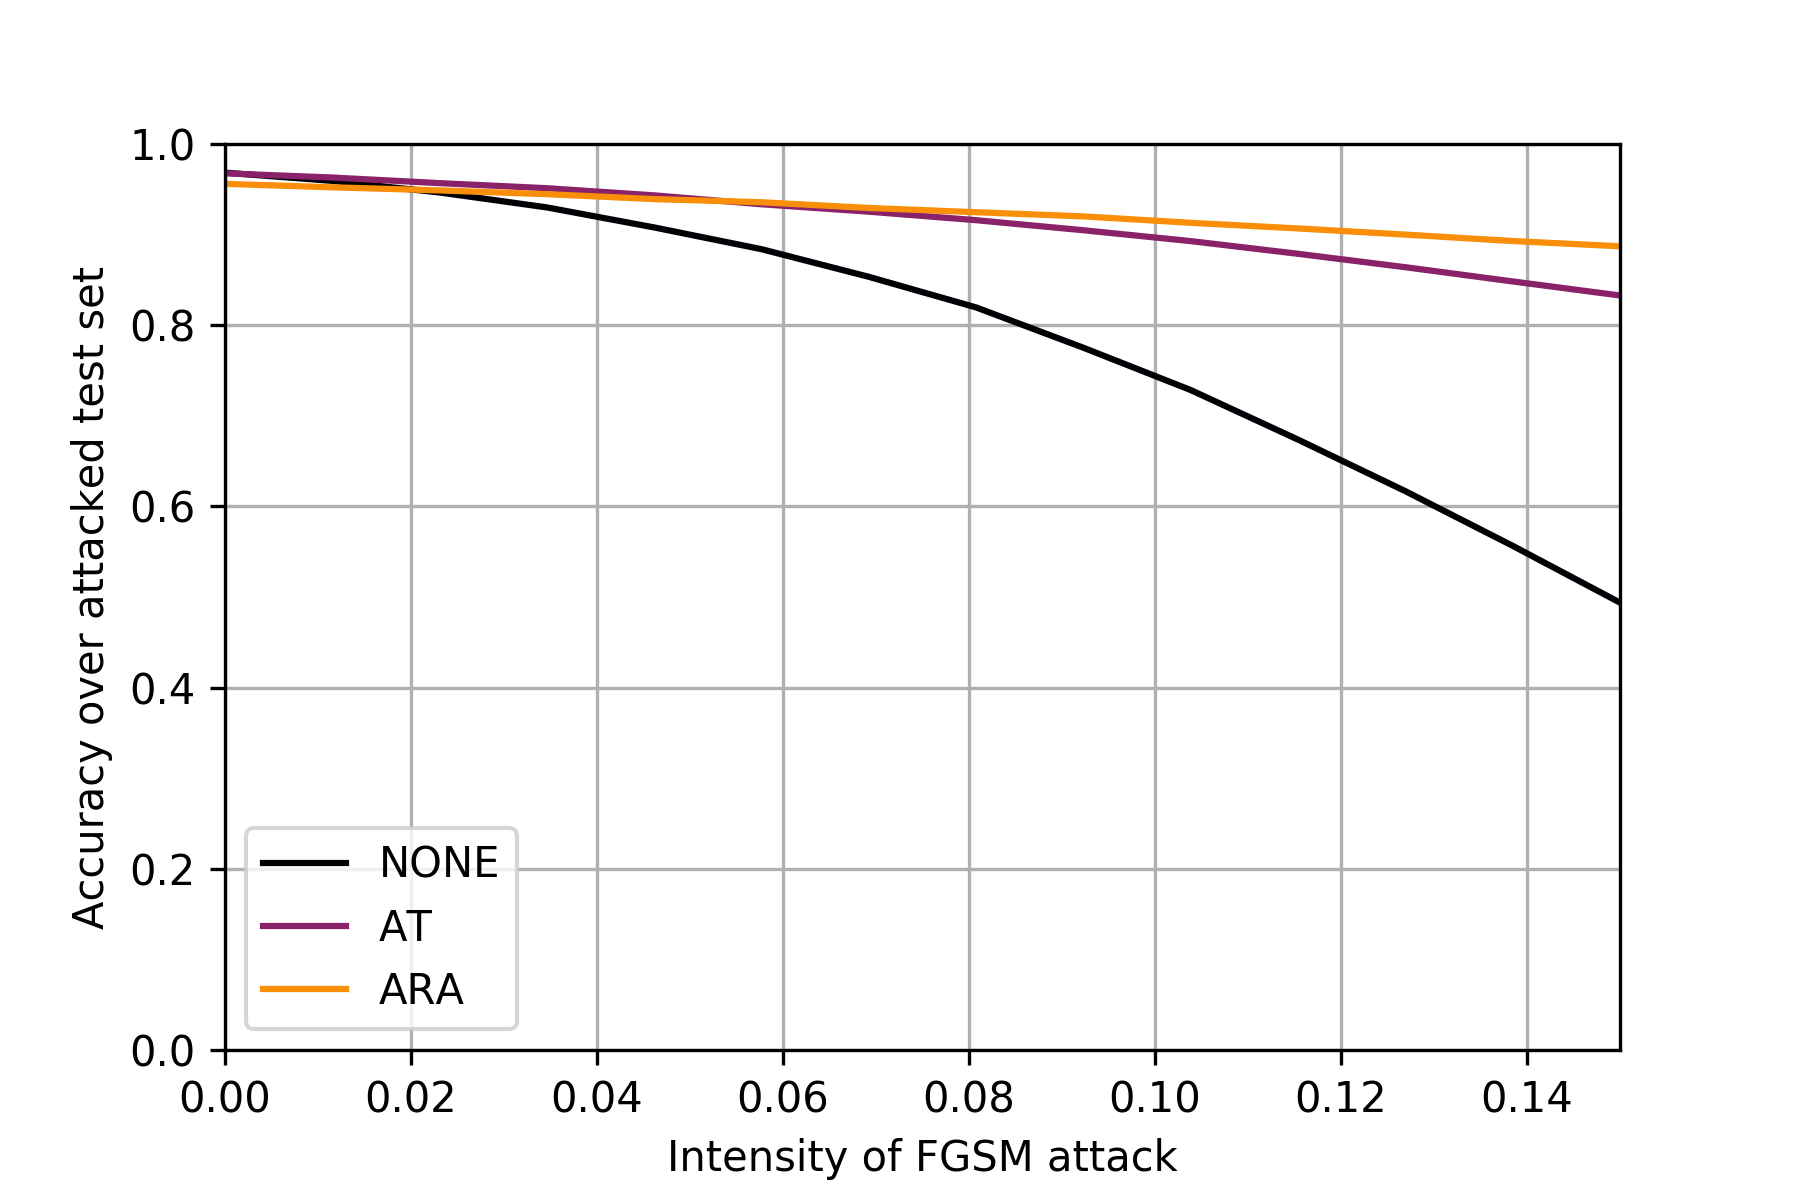
\includegraphics[width=\textwidth]{figures/comparison_mnist_fgsm.png}
        \caption{FGSM attack.}
        \label{fig:sub1}
    \end{subfigure}
     %add desired spacing between images, e. g. ~, \quad, \qquad, \hfill etc. 
      %(or a blank line to force the subfigure onto a new line)
    \begin{subfigure}[b]{0.45\textwidth}
        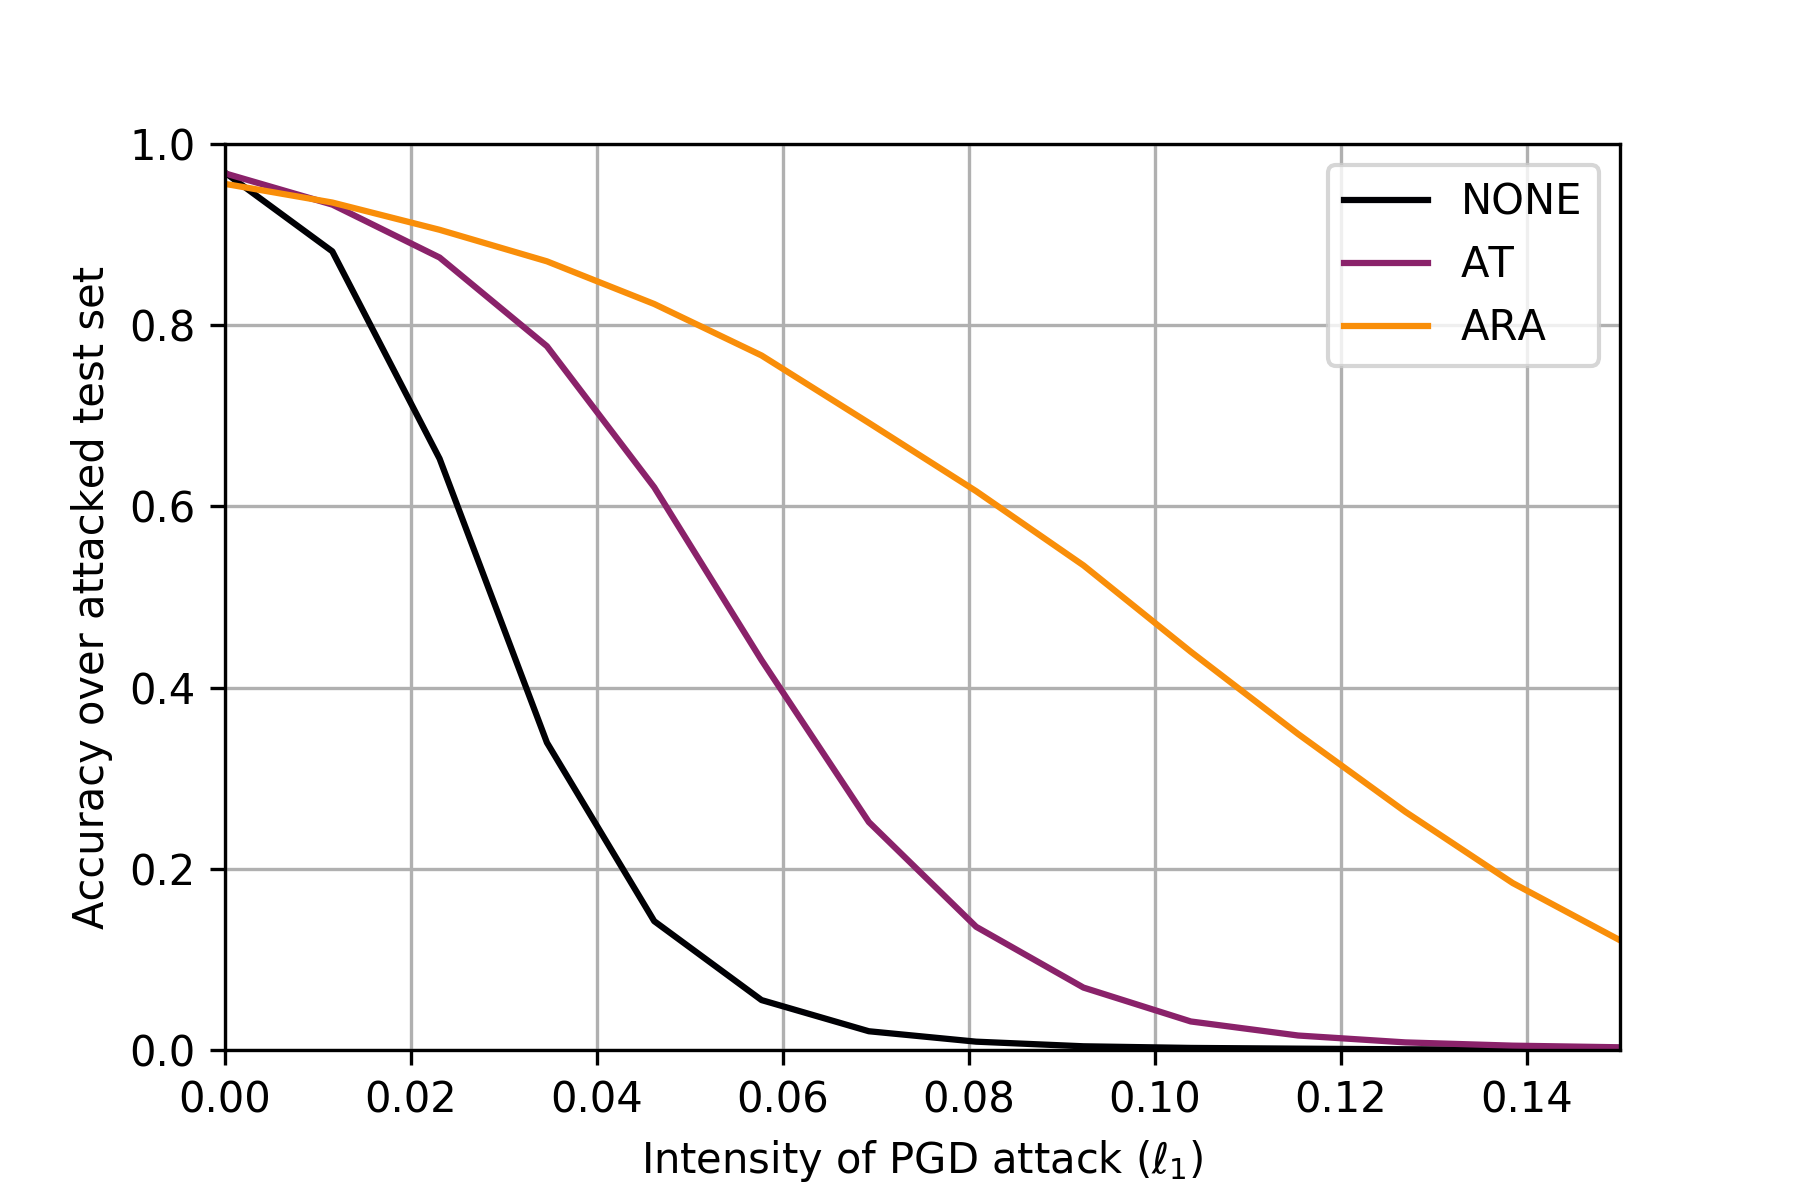
\includegraphics[width=\textwidth]{figures/comparison_mnist_pgdl1.png}
        \caption{PGD attack under $\ell_1$ norm.}
        \label{fig:sub2}
    \end{subfigure}
    \caption{Robustness of a deep network for MNIST under three defence mechanisms 
(none, AT, ARA). (a) depicts the security evaluation curves under the FGSM attack. (b) depicts the security evaluation curves under the PGD attack.}\label{fig:comparison_mnist}
\end{figure}
\fi

Figure \ref{fig:comparison_mnist} shows the \emph{security evaluation curves} \parencite{BIGGIO2018317} for three different defences (none, AT and ARA), using two attacks at test time: FGSM and PGD. Such curves depict the accuracy of the defender model at this task ($y$-axis), under different attack intensities $\alpha$ ($x$-axis). Note how the uncertainties provided by the ARA training method substantially improve the robustness of the neural network under both attacks. From the graphics, we observe that the ARA approach provides a greater degree of robustness as the attack intensities increase. This suggests that the proposed robustification framework can scale well to both tall and wide datasets and that the introduction of uncertainties by the ARA approach is highly beneficial to increase the robustness of the defended models.





%%%%%%%%%%%%%%%%%%%%%%%%%%%%%%%%%%%%%%%%%%%%%%%%%%%%
\section{Summary}

In this chapter, we studied the important problem of developing defences that protect ML models against malicious and intentional attacks and increase their robustness. We have surveyed how game theoretical approaches provide a framework to develop defence mechanisms, however they are not realistic since they are pervaded by common knowledge assumptions. We adopted ideas from Adversarial Risk Analysis to model several sources of uncertainty that the defender model may face, and proposed an enhanced robustification method. Experiments in spam detection and image classification show the benefits of the introduced framework.